%%
%% viQuantAgent / QuantAgent VN -- Academic Paper
%% Converted to the Elsevier elsarticle (numbered-citation) template,
%% based on elsarticle-template-num.tex, for submission to
%% Knowledge-Based Systems (KBS).
%%
%% FORMAT CONVERSION ONLY: the scientific content is unchanged from the
%% original cas-sc source (DKE_2026.tex); only front-matter markup and
%% class-specific macros (\credit, \printcredits, [pos=...] float
%% placement, \begin{keywords}, \tnotemark/\fnmark/\cormark, natbib
%% \citep) have been adapted to elsarticle conventions.
%%
\documentclass[preprint,12pt]{elsarticle}

\usepackage[
    left=1.8cm,
    right=1.8cm,
    top=2.0cm,
    bottom=2.0cm
]{geometry}

%% Use the option review to obtain double line spacing
%% \documentclass[authoryear,preprint,review,12pt]{elsarticle}

%% Use the options 1p,twocolumn; 3p; 3p,twocolumn; 5p; or 5p,twocolumn
%% for a journal layout -- left commented, preprint style is used here.
%% \documentclass[final,3p,times]{elsarticle}

%% For including figures, graphicx.sty has been loaded in elsarticle.cls.

%% The amssymb package provides various useful mathematical symbols
\usepackage{amssymb}
%% The amsmath package provides various useful equation environments.
\usepackage{amsmath}

%% Packages required by the original manuscript content (tables,
%% algorithms, float placement) -- preserved from the source document.
\usepackage[T1]{fontenc}
\usepackage[utf8]{inputenc}
\usepackage[vietnamese, english]{babel}
\usepackage{xcolor}
\usepackage{amsmath}
\usepackage{graphicx}
\usepackage{tabularx}
\usepackage{float}
\usepackage{placeins}
\usepackage{framed}
\usepackage[ruled,vlined,linesnumbered]{algorithm2e}
\usepackage{orcidlink}
\usepackage{hyperref}

\journal{Knowledge-Based Systems}

%% Figures live under figures/figs/... in this project; original
%% \includegraphics calls use the relative path "figs/..." as in the
%% source manuscript, so we add "figures/" to the graphics search path.
\graphicspath{{figures/}}

\begin{document}

\begin{frontmatter}

%% Title, authors and addresses

\title{Evaluating Quantitative Evidence in Multi-Agent Decision Support for Vietnamese Equities\tnoteref{t1}}
\tnotetext[t1]{This research is funded by Foreign Trade University under research program number FTURP02-2026-08.}

%% Authors
\author[1]{Hong-Viet Tran\,\orcidlink{0000-0002-4675-2123}}
\author[1]{Hoang-Dung Phan\,\orcidlink{0009-0003-6859-0852}}
\author[1,2]{Thanh-Tam Do Thi\,\orcidlink{0000-0002-7594-276X}}
\author[1]{Phuong-Thai Nguyen\,\orcidlink{0009-0006-2033-7788}}
\author[3]{Van-Tang Nguyen\,\corref{cor1}\orcidlink{0009-0009-7266-2437}}

%% Affiliations
\affiliation[1]{organization={Institute for Artificial Intelligence, University of Engineering and Technology, Vietnam National University},
            city={Hanoi},
            country={Vietnam}}

\affiliation[2]{organization={Faculty of Economic Information System and E-Commerce, Thuongmai University},
            city={Hanoi},
            country={Vietnam}}

\affiliation[3]{organization={Faculty of Technology and Data Science, Foreign Trade University},
            city={Hanoi},
            country={Vietnam}}

\cortext[cor1]{Corresponding author}


%% Abstract
\begin{abstract}
We examine quantitative evidence in a five-agent decision-support architecture for Vietnamese equities using an audit of archived predictions and an explicitly separate numerical-baseline reconstruction. The legacy benchmark contains 180 decisions across nine equities. Its Full branch achieves 65.0\% accuracy, below a constant DOWN/CASH rule at 68.9\%; balanced accuracy is 55.0\% and Matthews correlation is 0.113. The Base reports control, which removes both factors and sentiment, has balanced accuracy of 44.4\%. Mean independently compounded Full account return is negative, whereas CASH returns zero. Consequently, the Full--Base accuracy gap does not establish alpha information value or profitability. Additional train-fitted majority, momentum, logistic and factor-only baselines, together with continuous-hold and daily mark-to-market ledgers, are evaluated on a newly retrieved, frozen price snapshot. That snapshot differs from legacy at 74 of the 180 cycles and changes two labels, so these numerical results are not presented as a head-to-head comparison with archived Full predictions. Missing historical reports and training predictions also prevent verification of an identical-information comparator and a Full-exposure-matched control. The reanalysis documents class imbalance, target definitions, preprocessing boundaries and the remaining evidence needed before claiming predictive superiority.
\end{abstract}

%%Graphical abstract
\begin{graphicalabstract}
\centering
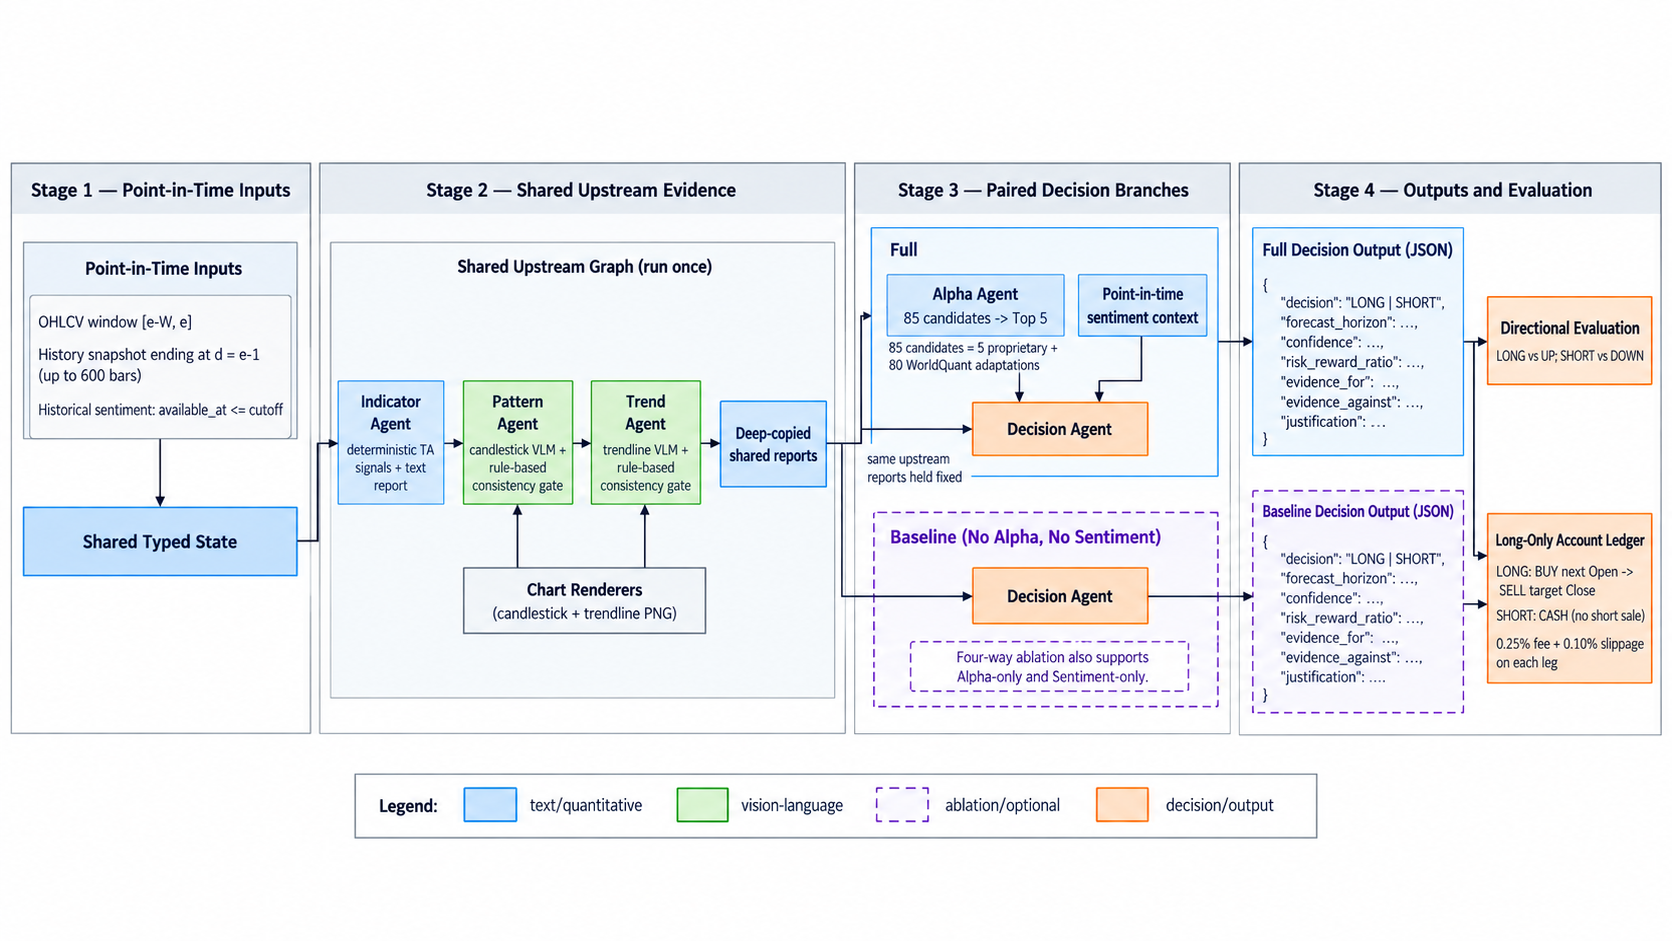
\includegraphics[width=0.95\textwidth]{figs/system_pipeline.png}
\end{graphicalabstract}

%%Research highlights
\begin{highlights}
\item A class-imbalance audit qualifies the legacy multi-agent benchmark.
\item Constant CASH exceeds legacy Full in raw accuracy and mean return.
\item Train-fitted numerical baselines use explicit temporal preprocessing.
\item Snapshot differences prevent a valid retrospective Full comparison.
\item The available evidence does not establish alpha value or profitability.
\end{highlights}

%% Keywords
\begin{keyword}
Multi-agent LLM \sep Knowledge fusion \sep Knowledge integration \sep Financial decision support \sep Alpha factor selection
\end{keyword}

\end{frontmatter}
% The elsarticle preprint footer exceeds its output box by 2.61pt.
% Visual inspection confirms no clipping; use a 3pt output tolerance.
\global\hfuzz=3pt

%% main text
\section{Introduction}
\label{sec:introduction}

Large language models (LLMs) have recently been used as reasoning engines in financial analysis. Their value for knowledge-based decision support depends on how quantitative, textual and visual evidence is represented and assessed, rather than on distributing tasks among agents alone. Frameworks such as QuantAgent \cite{xiong2025quantagent} provide a starting point for chart-based LLM decision support. Adapting such a framework to Vietnamese equities requires explicit treatment of Vietnamese-language news, single-asset factor inputs and the distinction between a directional forecast and a feasible cash-equity trade.

Vietnam motivates this implementation in three ways. First, the bar-count forecast horizon must be distinguished from entry, exit and settlement assumptions. Second, Vietnamese news requires a language-appropriate scorer, whose financial-domain validity still needs independent assessment. Third, OHLCV-only factor construction cannot retain the peer-relative meaning of every cross-sectional expression. These are practical adaptation questions, not evidence that the resulting system has solved emerging-market prediction.

We examine a concrete multi-agent implementation for Vietnamese equities. It combines deterministic technical-indicator reports, a native selector over 85 OHLCV factor candidates, Vietnamese sentiment scores, two chart-reading roles and a final binary Decision Agent. Indicator, Pattern, Trend and Decision roles and associated utilities reuse or modify QuantAgent components \cite{xiong2025quantagent}. The integration is an implementation and domain-adaptation exercise: condensed reports enter a prompt with heuristic evidence-priority instructions, rather than a learned knowledge-fusion representation.

Our question is how this implementation compares with class-aware and numerical controls on the same recorded historical market units, and what its archived executions can support about variability, components and economics. The primary comparison is Full versus Base. Base removes both selected-factor and sentiment sections, so this is a bundle contrast, not an isolated alpha-information treatment. A separate factorial panel includes factor-only, sentiment-only and matched-structure past-donor variants. Different prompt families and small repeated panels remain explicit rather than being pooled into a larger apparent experiment.

The completed release contains 102 main market units spanning six historical blocks and twelve selected dates, with 25 UP and 77 DOWN net labels. Full has pooled balanced accuracy (BA) of \FullBA\%, Base \BaseBA\%, and a price-only logistic comparator \LogisticPriceBA\%. CASH has higher ordinary accuracy than Full but BA of 50\%. Mean reference account returns are negative for Full and Base. These observations motivate an assessment of the implementation and its limits, rather than a claim of profitable trading or general predictive superiority.

The evaluation also exposes unresolved methodological defects. Native factor operations are isolated from prices after the outer decision cutoff in synthetic probes, but are not causal row by row within their trailing history. Native ranking and orientation diagnostics are in-sample. News availability and the sentiment classifier's financial-domain validity are not independently authenticated. We preserve these facts when reporting the frozen outputs. Separate train-fit numeric controls use causal adapters and cannot retrospectively repair the native LLM study.

The main contributions are as follows:
\begin{itemize}
\item A Vietnamese-equity adaptation that integrates an OHLCV factor selector and local-language sentiment with Indicator, Pattern, Trend and Decision roles. It extends reused chart-agent components through explicit quantitative and textual inputs rather than claiming a new learned fusion architecture.
\item A specified single-asset signal-construction method: 80 retained Formulaic Alpha adaptations and five custom handlers, top-five diagnostic ranking, and a separately represented time-decayed sentiment report. Its operator semantics and construction limits make the actual inputs distinguishable from idealised source formulas.
\item A shared-report evaluation design combining common-support baselines, repeated upstream and Decision executions, and five variants for factors, sentiment and a past donor. The comparison identifies which inputs differ without treating a bundled contrast as a causal alpha effect.
\item An empirical analysis linking class-aware prediction to transaction-cost-aware long-only accounts. On the main support, the Full--Base balanced-accuracy difference accompanies fewer false LONG forecasts and unchanged UP recall, while mean net returns remain negative. This distinguishes a classification change from demonstrated economic value.
\end{itemize}

Historical snapshots, actual requests/responses and metrics are retained with hashes for offline replay. The evidence is historical and exploratory: the reduced scope was amended after some inference, all outcome dates preceded the freeze, and the study does not establish causal component value or prospective deployment performance.

The remainder of this paper is organised as follows. Section~\ref{sec:relatedworks} reviews related work; Section~\ref{sec:formulation} formalises the task and signals; Section~\ref{sec:systemarchitecture} describes each agent; Section~\ref{sec:experimentalsetup} specifies the evaluation; Section~\ref{sec:backtestresults} reports results; Section~\ref{sec:limitations} discusses limitations and future work; and Section~\ref{sec:conclusion} concludes.

\section{Related work}
\label{sec:relatedworks}

\paragraph{Financial LLMs and chart agents}
Financial language models and adaptation frameworks include BloombergGPT and FinGPT \cite{wu2023bloomberggpt,yang2023fingpt}. TradingAgents organizes multiple financial analysis and decision roles \cite{tradingagents2024}. QuantAgent's version-specific architecture already includes Indicator, Pattern, Trend and Decision agents, shared state, chart rendering and trendline utilities \cite{xiong2025quantagent}. Our system reuses or modifies those elements; adding an alpha/sentiment path does not make the underlying chart-agent architecture novel. ChartLlama addresses multimodal chart understanding \cite{han2023chartllama}, while the cited Tsantekidis study concerns limit-order-book prediction, not candlestick-image recognition \cite{tsantekidis2017lob}. These tasks should not be treated as interchangeable validation of our chart reader.

\paragraph{Factor search and evaluation}
The source catalogue of 101 Formulaic Alphas describes expressions with cross-sectional and other requirements \cite{kakushadze2016formulaic}. Our 80 retained expressions are heuristic single-asset adaptations, with operators and deviations documented individually; five further formulas are custom to the implementation. Searching many candidates and choosing their orientation on the same history creates selection bias \cite{harvey2016}. Nested selection and assessment \cite{varma2006bias}, the Deflated Sharpe Ratio \cite{bailey2014deflated}, and White's Reality Check \cite{white2000reality} address related evaluation concerns. This study does not claim to have applied all those procedures: its auxiliary numeric study uses train-fit controls and a declared Holm family, while the native selector retains its audited defects.

\paragraph{Vietnamese sentiment and reproducibility}
ViSoBERT was developed for Vietnamese social-media language understanding \cite{nguyen2023visobert}. We use a distinct public 5CD-AI sentiment classifier derived from that backbone \cite{hf5cdsentiment}; its identity does not establish accuracy on Vietnamese financial news. General financial sentiment work such as FinBERT \cite{araci2019finbert} does not substitute for validating this classifier and corpus. Accordingly, we report the implemented scoring recipe, availability and provenance rather than assuming financial-domain competence. Exact hosted-model replay poses an additional limitation: the text model's published description \cite{openai2025gptoss} does not identify the immutable weights served for an archived request. We retain observed aliases and fingerprints without treating them as weight attestations.

\section{Problem Formulation}
\label{sec:formulation}

\subsection{Market Model and Data}
For each security $s$ in the declared universe $\mathcal{S}$, let $\mathbf{x}_u=(O_u,H_u,L_u,C_u,V_u)$ denote one observed OHLCV bar at zero-based position $u$. Positions index vendor observations, not consecutive calendar days. The evaluated chart window has $W=45$ bars and exclusive end $e$:
\begin{equation}
 \mathbf{X}_e=(\mathbf{x}_{e-W},\ldots,\mathbf{x}_{e-1}),
 \qquad d=e-1,\qquad h=e-1+L.
 \label{eq:time_index_contract}
\end{equation}
The last visible bar is $d$, entry is planned at $e$, and the candidate exit is at $h$. Thus neither entry nor exit prices belong to the visible chart. The alpha path separately receives a historical prefix ending at $d$, up to 600 observed bars. These two history requirements should not be conflated. Weekends, holidays and vendor gaps do not create synthetic bars; incomplete target spans are rejected.

Price/volume fields retain the reconstructed vendor units and adjustment conventions. Missing-volume handling in the native implementation can substitute intrabar range as a proxy; its whole-frame branch is one source of the row-wise causal defect described below. A numerical proxy does not authenticate actual turnover, transaction VWAP or market depth. Dataset eligibility and the BHN exclusions are defined in Section~\ref{sec:experimentalsetup}.

\subsection{Directional Prediction Task}
Let $d$ be the last observed session at a decision cutoff, $e=d+1$ the planned entry session, and $L=3$. The candidate LONG cycle buys at $Open_e$ and exits at $Close_{e+L-1}=Close_{d+3}$. Thus three observed bars include the entry bar, and exit is two observed sessions after entry. With brokerage $f=0.0025$ and slippage $s=0.001$ on each leg, the target is
\begin{equation}
 r^{net}_d=\frac{Close_{d+3}}{Open_{d+1}}
 \frac{(1-f)(1-s)}{(1+f)(1+s)}-1,
 \qquad y_d=\mathbf{1}[r^{net}_d>0].
 \label{eq:netlabel}
\end{equation}
UP means a strictly positive candidate LONG net return; zero belongs to DOWN. Gross return is a separate diagnostic on the same net-elicited predictions, not a replacement label or an additional inference experiment. The seven gross/net label disagreements are retained. Decision Close differs from entry Open at 65 of the 102 units, so a close-to-close label is not equivalent.

The agent chooses LONG or SHORT. In the long-only reference ledger, LONG allocates the account to the cycle and SHORT holds CASH; SHORT is not a short sale and a correct DOWN classification earns no bearish trading return. Account return therefore differs from the candidate-LONG target. Missing horizons are rejected rather than shortened. Canonical exports distinguish decision Close, entry Open and exit Close. A legacy field called \texttt{actual\_prev\_close} is not authenticated as decision Close merely because it sometimes equals entry Open; its unresolved semantic provenance is preserved in the legacy audit.

\subsection{Alpha Factor Formalisation and Adaptation}
At each outer cutoff the native implementation receives a 600-session historical prefix and selects five of 85 candidates. Eighty are retained WorldQuant adaptations and five are custom formulas. The companion registry gives every source expression, handler, operator window, ties/fills and excluded expression; it does not assert mathematical equivalence to the source catalogue \cite{kakushadze2016formulaic}. Among 21 exclusions, 17 involve industry neutralization, one market capitalization, and three price/volume omissions have no authenticated selection rationale. They are not all described as impossible cross-sectional translations.

A registered function maps features constructed from the available history to a sequence of factor values. Replacing a cross-sectional rank by a rolling rank changes the question from comparison with peers to comparison with the asset's own past. The native rank implementation counts preceding values strictly below the current value, so ties do not contribute as lower values. Partial windows and the source expression's explicit time-series lookbacks remain operator-specific. This heuristic localisation is not an invariance-preserving derivation of the source formula.

Let $a^{(k)}_{u,d}$ be the normalized value for candidate $k$ at row $u$ as computed from the prefix ending at $d$. The second index is intentional: whole-Series normalization may change a historical row when the prefix changes. A zscore--tanh path has the form
\begin{equation}
 a^{(k)}_{u,d}=\tanh\!\left(\frac{\alpha^{(k)}_u-\mu_{k,d}}{\sigma_{k,d}+\epsilon}\right),
 \label{eq:alpha_norm}
\end{equation}
where the location and scale are derived from the supplied Series, not necessarily a training-only fit independent of each row. Min--max and rank-based alternatives also exist. Equation~\ref{eq:alpha_norm} illustrates one implemented transform, rather than claiming that every candidate uses one identical causal normalization. ADV is mean share volume over the specified lookback and the daily VWAP proxy uses typical price; neither adds missing cross-sectional information.

\subsection{Walk-Forward Alpha Selection}
Native candidate diagnostics use the trailing sample to estimate rank correlation (IC), sign orientation, directional accuracy and a signed-return Sharpe proxy, then rank a weighted composite. IC orientation and factor selection are consequently in-sample diagnostics, not independent factor discoveries. The normalization names include zscore--tanh, min--max and rank-based transforms; the actual whole-Series implementations, partial windows, denominator guards and NaN/zero fills matter more than their nominal names. Returns are implemented as percentage changes, and VWAP/ADV use OHLCV proxies rather than independently measured transaction VWAP or dollar volume.

The default score is $0.40\,m(|IC|)+0.35\,m(Accuracy)+0.25\,m(Sharpe)$, where $m$ is min--max scaling across candidate diagnostics (a constant range maps to 0.5). Negative IC reverses the signal used for diagnostic accuracy and the signed-return proxy; displayed diagnostic rounding precedes ranking. Directional accuracy uses the strong-signal subset $|a|>0.05$, with fallback conventions for insufficient support. The signed-return Sharpe proxy is not a realized long-only CASH ledger. The nominal minimum-history check is not a causal warm-up trim: partially filled early rows can enter native diagnostics. Exact metric guards and tie/sort behaviour remain in the registry implementation rather than being replaced with an idealized formula.

For clarity, write $\mathcal{T}_{k,d}$ for the finite historical sample entering a candidate's diagnostics, and $r^{net}_u$ for the corresponding candidate-LONG net target. The rank-correlation diagnostic and orientation are
\begin{equation}
 IC_{k,d}=\operatorname{SpearmanCorr}(a^{(k)}_{u,d},r^{net}_u)_{u\in\mathcal{T}_{k,d}},
 \qquad o_{k,d}=\begin{cases}-1,&IC_{k,d}<0,\\1,&\text{otherwise}.\end{cases}
 \label{eq:ic}
\end{equation}
Oriented signal signs enter historical accuracy on the strong-signal subset and the signed-return proxy. Those diagnostics and the top-five choice reuse the same trailing observations. They are therefore selection statistics, even when the current entry and exit bars are outside the supplied prefix. The actual code's finite-support guards, default values and rounding are preserved in the registry audit.

For eligible candidates $\mathcal{V}_d$, min--max scaling of diagnostic $q$ is
\begin{equation}
 m_d(q_k)=\begin{cases}
 (q_k-q_{min})/(q_{max}-q_{min}),&q_{max}-q_{min}\ge10^{-9},\\
 0.5,&\text{otherwise},
 \end{cases}
 \label{eq:candidate_minmax}
\end{equation}
where the extrema are over $\mathcal{V}_d$. The native ranking is
\begin{equation}
 S_{k,d}=0.40m_d(|IC_{k,d}|)+0.35m_d(Accuracy_{k,d})+0.25m_d(Sharpe_{k,d}),
 \label{eq:composite}
\end{equation}
and the five highest eligible scores supply the current report. The quantity named Sharpe in this selector is a signed-return ranking proxy, not the long-only account Sharpe. Its inclusion does not demonstrate factor profitability. Causal train-fit fixed/dynamic/random controls are a separate study in Section~\ref{sec:backtestresults}.

\textbf{The native row-wise causal gate fails.} Counterexamples show that \texttt{delay().bfill()}, whole-Series normalization and the full-frame volume-availability branch can change earlier row values when later rows are extended or altered. In contrast, synthetic outer-cutoff probes found that poisoning data after the supplied 600-bar prefix did not change the native outputs. These are different properties: cutoff isolation in a fixture does not make all rows within the prefix causal, certify news PIT, or remove selection bias. We have not repaired the historical native inputs and then attributed the same saved LLM outcomes to a corrected mechanism.

Custom definitions are summarized in \ref{app:signals}. For example, native BFE uses $\tanh(1.5(\%B-0.5)VolZ_5)$: negative volume z-score reverses the sign and zero cancels it. There is no volume-expansion or squeeze gate. Native registry and prototype/fallback paths have different preprocessing, including sample versus population SD and rounded technical variables. A selected-factor display rank is not a permanent factor ID. Six selected metadata slots on six main units disagree with handler descriptions; the affected actual prompts did not contain the literal wrong formula. Their semantic effect on the LLM has not been measured separately. Handler identity, descriptions and frozen outcomes remain distinguishable.

\subsection{Sentiment Signal Construction}
The archived local scoring recipe identifies \texttt{5CD-AI/Vietnamese-Sentiment-visobert} at revision \texttt{d7738b85200272f10ba8b048d80236c8c582b581}, with labels NEG/POS/NEU and article score $P(POS)-P(NEG)$. Tokenization uses an explicit 256-token limit, batch size eight, padding and truncation; tokenizer checks and saved probability/score checks do not constitute a new model evaluation. The released scorer is distinct from the ViSoBERT backbone citation \cite{nguyen2023visobert,hf5cdsentiment}.

Availability requires at least three distinct identities with explicit accepted scorer provenance and finite scores in a 90-day cutoff window. Date-only publication is conservatively made available the following day; explicit availability metadata is retained. For eligible articles, the frozen aggregate is
\begin{equation}
 S_d=\frac{\sum_i 2^{-age_i/30}\,[P_i(POS)-P_i(NEG)]}{\sum_i 2^{-age_i/30}},
 \label{eq:sentiment}
\end{equation}
with age in days at the cutoff, hence a 30-day half-life. Missing sentiment is not an observed zero/neutral signal. The frozen provider supplies the aggregate/count report but empty article-detail and peer lists to the normalizer; its z-score and relative fields are therefore zero on this path, not independently observed peer information. The normalizer's reliability flag uses at least eight articles, distinct from the three-article availability rule. A false reliability flag alone does not mean the weighted report was missing. We do not substitute the prototype sentiment equations for these actual inputs.

Legacy inventory contains 180 article records and 177 unique identities, not 8,180 authenticated articles. All 180 legacy scorer identities are unknown; under the corrected strict eligibility/provenance rule none of the 180 legacy test cutoffs has three valid articles. Old runtime counts, duplicate memberships and article counts are retained separately from this strict audit. The reconstructed study and 154 locally rescored excerpts are a separate provenance scope. Actual prompt audits establish which sections were delivered, not that the news content was historically available or correctly interpreted. The authors have no independently labelled financial-news validation set. Social-media domain mismatch and unauthenticated content/publication availability preclude financial-domain accuracy and PIT-certified sentiment claims.


\subsection{Multi-Agent Decision Function}
Let $R^I_d,R^P_d,R^T_d$ be the Indicator, Pattern and Trend reports shared within a pair, and let $R^A_d,R^S_d$ denote the factor and sentiment sections. With variant mask $v=(v_A,v_S)$, the implemented decision can be written
\begin{equation}
 \widehat y_{d,v}=\mathcal{D}_{\theta}\!\left(\operatorname{distill}(R^I_d,R^P_d,R^T_d),
 v_A R^A_d,v_S R^S_d;\pi_v\right),
 \label{eq:decision_function}
\end{equation}
where the products indicate inclusion/omission of text sections, not numerical multiplication. $\pi_v$ includes formatting and evidence-priority instructions. Main Full uses $(1,1)$ and Base $(0,0)$; factorial A/S/AS use $(1,0)/(0,1)/(1,1)$, and P replaces the factor values using the frozen donor rule. This notation describes prompt composition, not a learned fusion layer. Confidence and risk/reward fields are model statements and are not calibrated probabilities or independently executed orders.

\subsection{Walk-Forward Evaluation Protocol}
The evaluation visits the frozen list of eligible cutoffs in chronological order within each account scope. It does not run a new uniform three-bar grid across the entire price history. At each cutoff the common inputs and report parents are retained, and each registered variant yields its recorded prediction. Only subsequently are predictions joined to the immutable net target and reference account ledger. The following algorithm describes this paired historical protocol; it does not certify row-wise causality of the native selector.

\par\medskip\noindent\fbox{\begin{minipage}{0.95\linewidth}
\refstepcounter{algorithm}\label{alg:walkforward}
\textbf{Algorithm \thealgorithm. Shared-report historical evaluation}
\begin{enumerate}
\item Read the frozen eligible unit list and chronological train/validation/test masks; reject incomplete windows or horizons.
\item At $d=e-1$, retain the 45-bar chart window, historical factor prefix, sentiment provenance and their exact hashes.
\item Compute Indicator/factor reports and obtain the recorded Pattern/Trend reports. Retain upstream identity for the pair.
\item Compose each registered variant from the shared reports, enabled factor/sentiment sections and the correct prompt family.
\item Retain its actual request, successful output, errors/order/epoch and checkpoint; never choose an outcome by test performance.
\item Join saved LONG/SHORT forecasts to the common net labels. Map SHORT to CASH in each separate account.
\item Report pooled/macro/support-aware classification, paired block diagnostics and account outcomes on their declared scopes.
\end{enumerate}
\end{minipage}}\par\medskip

Under the fractional reference ledger, a non-overlapping cycle with LONG indicator $\ell_j$ updates wealth by $W_{j+1}=W_j(1+\ell_j r^{net}_j)$, while a CASH cycle leaves wealth unchanged. This product applies to each account and its reference assumptions; settlement/capacity sensitivities retain explicit receivables and residual holdings instead of being replaced by this shorthand. Account means across securities are not portfolio wealth.

\section{System architecture}
\label{sec:systemarchitecture}
\subsection{Overview}
The implementation uses a LangGraph directed graph with five specialised roles and a shared typed state. Indicator, Pattern, Trend and Decision roles, shared state, chart tools and trendline procedures reuse or modify QuantAgent components; the upstream MIT notice is preserved in the repository \cite{xiong2025quantagent}. Alpha adds numerical factor and Vietnamese sentiment reports. This integration is an engineering adaptation, distinct from inventing the inherited graph or validating a learned knowledge-fusion method.

Figure~\ref{fig:flow} shows the actual information flow. In the evaluated backtest, Indicator is deterministic and the numerical/report Alpha path bypasses an additional alpha-reasoning LLM call. Pattern and Trend consume their separate chart images, while Decision receives the condensed reports and enabled quantitative/text sections. The five role names consequently do not imply five hosted LLM calls per forecast. Model aliases and actual request accounting are specified in Section~\ref{sec:experimentalsetup}.

\begin{figure}[!htbp]
\centering
% Sơ đồ vai trò thực chạy; không biểu diễn learned fusion hoặc causal gate đã đạt.
\begin{tikzpicture}[
  role/.style={draw,rounded corners,align=center,text width=2.6cm,minimum height=0.85cm,font=\small},
  link/.style={-{Latex[length=2mm]},thick}]
\node[role,fill=gray!10] (price) at (0,-1.3) {Frozen OHLCV\\600-bar prefixes\\45-bar charts};
\node[role,fill=gray!10] (news) at (0,-3.9) {Frozen news scores\\Domain/PIT validity\\not established};
\node[role] (ind) at (4,0) {Indicator\\Deterministic report};
\node[role] (pat) at (4,-1.3) {Pattern\\Vision report/replay};
\node[role] (trend) at (4,-2.6) {Trend\\Corrected chart/report};
\node[role] (alpha) at (4,-3.9) {Alpha role\\Numeric factors and\\sentiment context};
\node[role,fill=blue!5,minimum height=1.6cm] (prompt) at (8,-1.9) {Shared I/P/T reports\\Enabled sections\\Heuristic prompt\\instructions};
\node[role] (decision) at (12,-1.9) {Decision LLM\\Structured LONG\\or SHORT};
\node[role,fill=gray!10] (ledger) at (12,-3.9) {Account simulation\\SHORT maps to CASH};
\draw[link] (price.east) -- (ind.west);
\draw[link] (price.east) -- (pat.west);
\draw[link] (price.east) -- (trend.west);
\draw[link] (price.east) -- (alpha.west);
\draw[link] (news.east) -- (alpha.west);
\draw[link] (ind.east) -- (prompt.west);
\draw[link] (pat.east) -- (prompt.west);
\draw[link] (trend.east) -- (prompt.west);
\draw[link,dashed] (alpha.east) -- (prompt.south west);
\draw[link] (prompt.east) -- (decision.west);
\draw[link] (decision.south) -- (ledger.north);
\node[align=center,font=\small,text width=4.3cm] at (8,-3.9) {Base omits factor and sentiment sections;\\no learned fusion module};
\end{tikzpicture}

\caption{System pipeline with shared-report Full/Base comparison. Indicator and alpha backtest reports are deterministic/numerical; Pattern and Trend use vision requests. Decision aggregates enabled reports by prompt instructions.}
\label{fig:flow}
\end{figure}

\subsection{Indicator Agent}
Indicator Agent computes and renders five deterministic TA-Lib-based votes: MACD(12,26,9), RSI(14), Stochastic(14,3,3), Williams \%R(14) and ROC(10). They are momentum/trend indicators, not five volatility oscillators. Its backtest node returns a report and messages, without calling an LLM or forwarding the declared state schema's complete numeric arrays. Bollinger variables can be computed on the alpha path; BB/ADX state declarations do not create two additional Indicator votes. \ref{app:indicator_logic} specifies the ordered boundaries and missing-data convention \cite{talib_rsi_docs,talib_willr_docs}.

Four-decimal rounding precedes classification, nonfinite samples are removed and zero is retained. Crossovers take priority where specified; overlapping RSI/Williams thresholds require ordered branches rather than two simultaneous unconditional rules. Each missing/error result contributes a neutral vote within the fixed denominator of five. Directional plurality and the confidence categories are deterministic summary heuristics. They are not calibrated probabilities, and an immutable signal tally does not make a downstream narrative correct.

\subsection{Alpha Agent}
\paragraph{Alpha selection}
The Alpha role evaluates 85 native candidates: 80 retained WorldQuant adaptations and five custom formulas. It supplies a selected top-five report from the trailing prefix, using the diagnostic score in Eq.~\ref{eq:composite}. The transformations, metric support, IC orientation and native row-wise causal failure are defined in Section~\ref{sec:formulation}. A rolling own-history rank is not a cross-sectional rank, and the 21 exclusions are not all justified by an inability to translate cross-sectional operators. Full expressions and exception handling remain in the registry; \ref{app:signals} gives the custom formulas needed to read the reports.

Selection, IC sign and candidate diagnostics reuse trailing observations. Hence the current value is an input to a report, while the reported skill fields are in-sample ranking statistics. Neither choosing the top five nor reversing negative IC establishes out-of-sample profitability. Six selected metadata slots have description/handler mismatches; actual prompts, metadata and implementation identity are kept distinct. No historical prediction is repaired to agree with a corrected description.

\paragraph{Sentiment integration}
Vietnamese sentiment is a separate contextual report, not an input to the native OHLCV factor formulas or score. The frozen provider supplies aggregate/count information and empty article-detail/peer lists. Relative sentiment and z-score fields on that path are consequently zero-valued outputs of the normalizer, rather than measured contemporaneous peer evidence. The three-article availability rule differs from the eight-article reliability flag. The 90-day window, 30-day decay, scorer revision and provenance limitations are specified in Section~\ref{sec:formulation}.

Figure~\ref{fig:alpha_agent} separates OHLCV factor selection from sentiment-context construction and shows the information delivered by the evaluated backtest. Optional live endpoints, lexicon fallbacks and peer discovery are repository capabilities; they are not evidence that the corresponding inputs were used or historically available in the evaluated calls.

\begin{figure}[!htbp]
\centering\begin{tikzpicture}[x=1cm,y=1cm,>=Latex,
 box/.style={draw=blue!55!black,fill=blue!4,rounded corners,align=center,text width=6.4cm,minimum height=1.2cm,font=\footnotesize},
 sent/.style={box,draw=green!40!black,fill=green!4},
 endbox/.style={draw=orange!65!black,fill=orange!7,rounded corners,align=center,text width=13.7cm,minimum height=1.2cm,font=\footnotesize},
 arr/.style={->,thick}]
\node[font=\bfseries] at (0,1.1) {Native OHLCV path};
\node[font=\bfseries] at (7.3,1.1) {Separate frozen sentiment path};
\node[box] (a1) at (0,0) {Prefix ending at decision $d$\\Up to 600 observed bars};
\node[box] (a2) at (0,-1.8) {85 native candidates\\80 adaptations + five custom handlers};
\node[box] (a3) at (0,-3.6) {Finite-support diagnostics and IC sign\\Same trailing sample; in-sample selection};
\node[box] (a4) at (0,-5.4) {Weighted score; select top five\\Native row-wise causal defect remains};
\node[box] (a5) at (0,-7.2) {Factor report / skill fields\\Compact or explicit-five-row family};
\node[sent] (s1) at (7.3,0) {Saved article scores and provenance\\Historical availability unverified};
\node[sent] (s2) at (7.3,-1.8) {90-day cutoff window; distinct identities\\At least three valid records for availability};
\node[sent] (s3) at (7.3,-3.6) {Probability difference / weighted mean\\30-day decay half-life};
\node[sent] (s4) at (7.3,-5.4) {Aggregate/count report\\No observed peer/article-detail comparison};
\node[sent] (s5) at (7.3,-7.2) {Separate sentiment text / missingness\\Reliability $\ge8$ is a different flag};
\node[endbox] (o) at (3.65,-9.3) {Variant-enabled sections enter Decision; sentiment does not enter native factor formulas.\\No extra Alpha reasoning-model call on this backtest path.};
\foreach \p/\q in {a1/a2,a2/a3,a3/a4,a4/a5,s1/s2,s2/s3,s3/s4,s4/s5}{\draw[arr] (\p)--(\q);}
\draw[arr] (a5.south)--(a5.south |- o.north);
\draw[arr] (s5.south)--(s5.south |- o.north);
\end{tikzpicture}

\caption{Alpha Agent: native OHLCV selection and separate sentiment context. Native factor diagnostics retain their causal/selection defects; the frozen sentiment path has no authenticated peer comparison. Both reports enter Decision only when enabled by the variant.}
\label{fig:alpha_agent}
\end{figure}

\subsection{Pattern Agent}
Pattern Agent analyses a candlestick PNG rendered from the exact 45-bar window. The prompt requests a chart formation, recent-candle evidence, directional bias, confidence and trading implication. The report parser retains the structured text fields; format completion and consistency checks are distinguished from financial correctness. Figure~\ref{fig:charts} presents an actual archived chart pair rather than a synthetic demonstration.

Candle bodies are green when Close exceeds Open and red otherwise, including a doji. This is an Open--Close body rule, not the Vietnamese exchange board's reference-price colouring rule. The exchange-board convention is not used to infer candle direction. After inference, consistency rules compare the claimed bias with simple OHLCV-derived properties such as the final body and recent closes. A contradiction flag can reduce displayed confidence; it cannot reveal which candle the VLM actually attended to. Alternative text-only paths in the general application are not assumed to have replaced any frozen vision input.

\begin{figure}[!htbp]
\centering
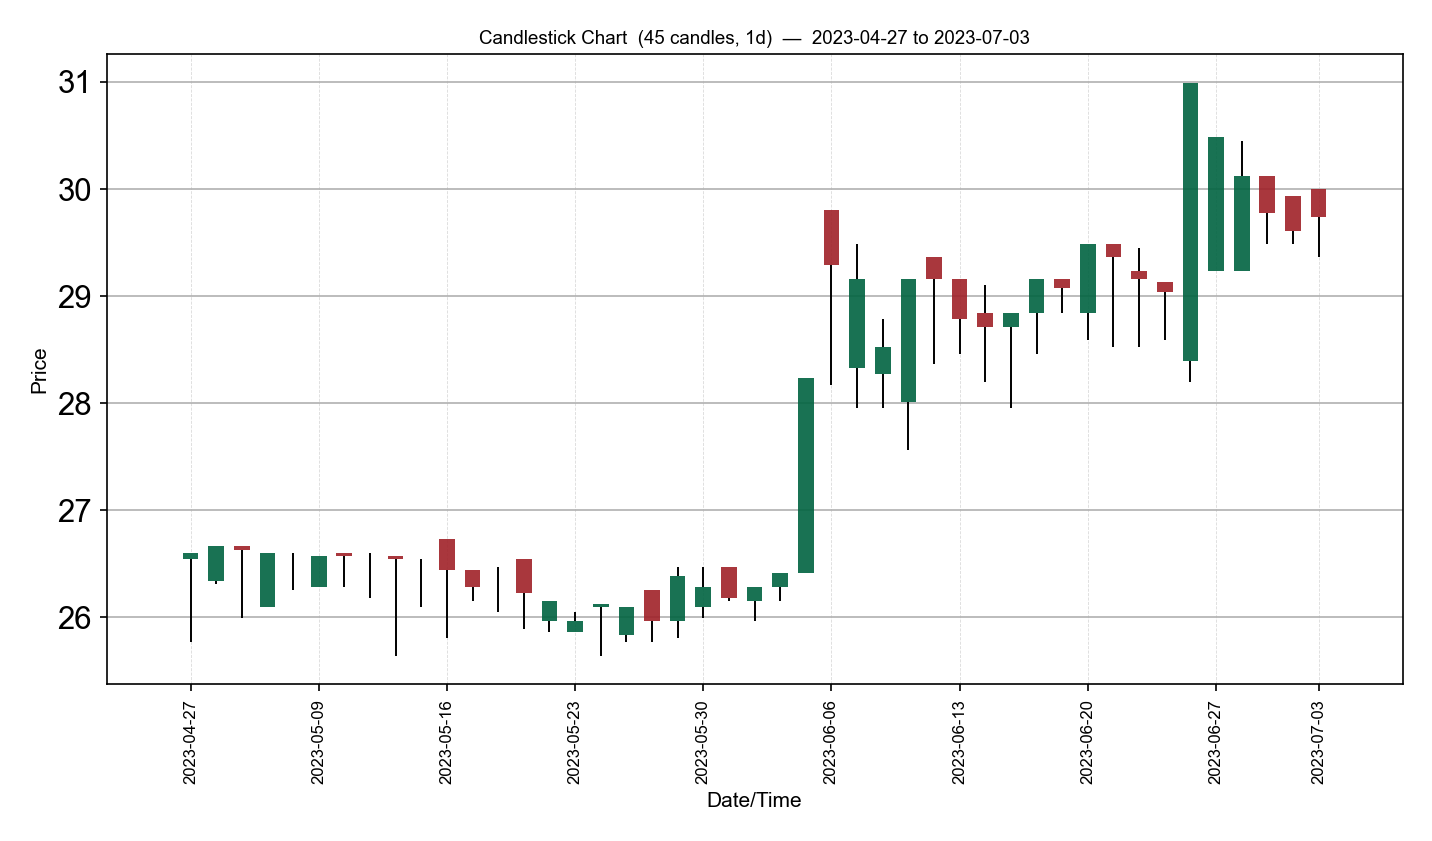
\includegraphics[width=0.90\textwidth]{figs/final_pattern.png}\par\smallskip
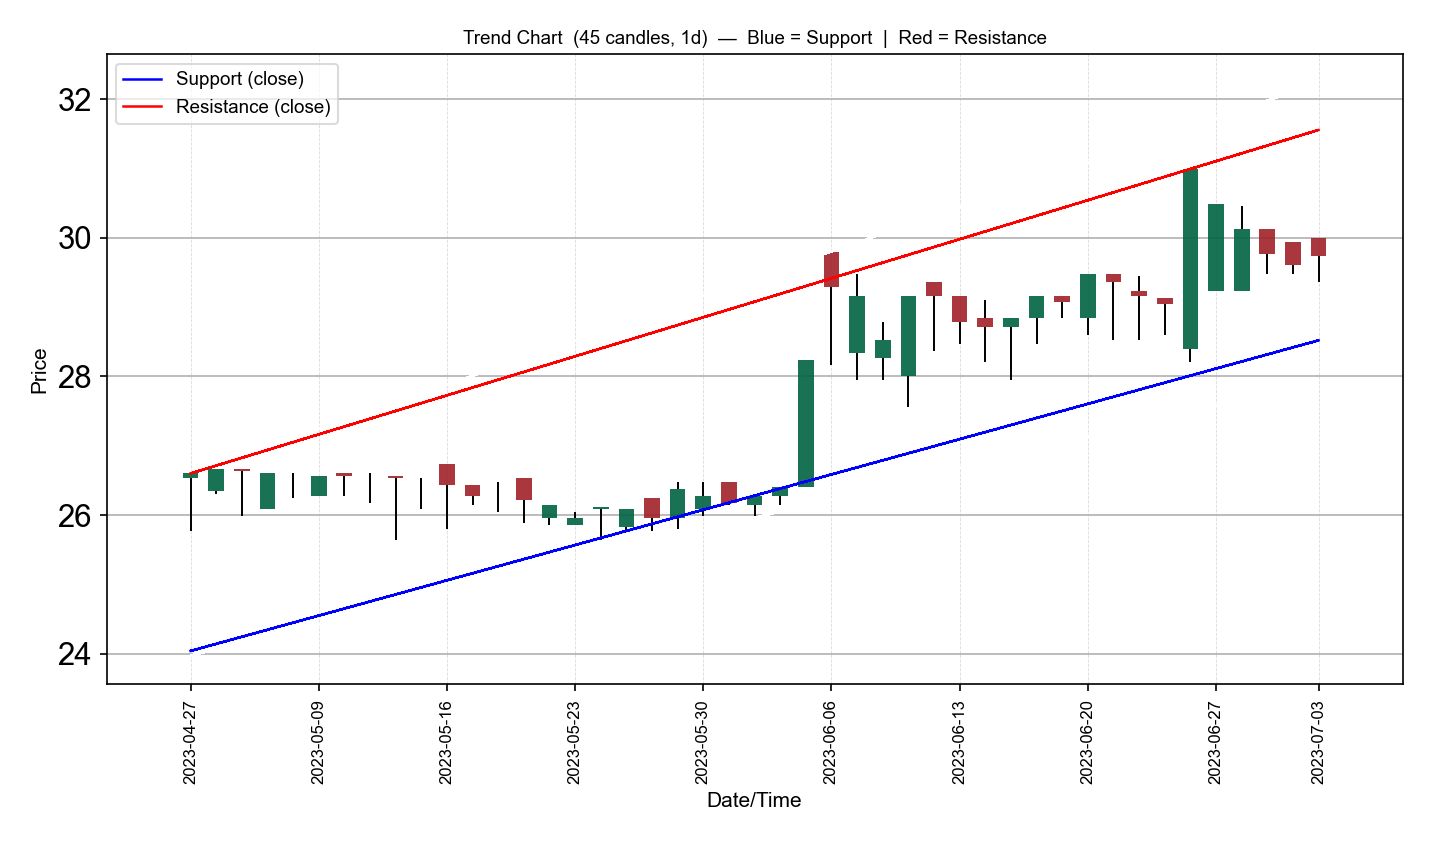
\includegraphics[width=0.90\textwidth]{figs/final_trend.png}
\caption{Actual Pattern and corrected Trend inputs for CMG on 3 July 2023, the first chronologically eligible main unit. Bodies compare Close with Open; the Trend legend maps blue to support and red to resistance. The unit was selected by date then symbol/ID without inspecting outcomes.}
\label{fig:charts}
\end{figure}

\subsection{Trend Agent}
Trend Agent receives a separate chart with fitted support/resistance lines. The inherited fitting utility starts with a least-squares close-price line, selects upper/lower deviation pivots, and optimizes a slope through each pivot under a non-crossing constraint. It implements both a close-only channel and a high/low channel, the latter using close-price regression to find pivots and high/low data for the bounds. These are numerical lines over the supplied window, not human-verified latent support levels.

For row position $u$, a fitted line has form $b+mu$. A support bound must remain below the corresponding price sequence within the implementation tolerance; resistance must remain above it. The local slope search reduces its step when the squared-deviation objective fails to improve or violates the constraint. The VLM then describes direction, levels, slope, price relative to support, forecast and confidence. Support is drawn blue and resistance red. A deterministic consistency check against simple price/trend summaries does not validate every reported level or coordinate.

The renderer audit matched 204 images across 102 units byte for byte and pixel for pixel, and 240 actual vision requests matched their image caches and Vietnamese templates. It verified body geometry, colour and legend handles, not the model's visual understanding. In particular, the Vietnamese word \emph{xanh} is less colour-specific than the corrected English ``blue'' wording. Inherited high-frequency/K-line prompt language also remains distinguishable from this daily-bar application. Matched local-pattern interventions and trend swaps would be needed to test whether the model uses the purported visual evidence.

\subsection{Decision Agent}
Decision receives condensed Indicator, Pattern and Trend reports plus enabled factor/sentiment sections. Reports are distilled and capped before prompt composition. The observed successful Decision prompts are at most 4,187 characters, below the 6,500-character guard. Figure~\ref{fig:decision_agent} shows report composition, prompt instructions, structured output and the separate action mapping.

\begin{figure}[!htbp]
\centering\begin{tikzpicture}[x=1cm,y=1cm,>=Latex,
 box/.style={draw=blue!55!black,fill=blue!4,rounded corners,align=center,text width=6.5cm,minimum height=1.8cm,font=\footnotesize},
 act/.style={box,draw=orange!65!black,fill=orange!6},arr/.style={->,thick}]
\node[box] (r) at (0,0) {\textbf{1. Shared reports}\\Indicator / Pattern / Trend\\Enabled factor/sentiment text};
\node[box] (p) at (7.6,0) {\textbf{2. Distil and compose prompt}\\Observed maximum: 4,187 characters\\Guard: below 6,500 characters};
\node[box] (i) at (0,-2.9) {\textbf{3. Evidence-priority instructions}\\Trend/candles; then momentum\\Enabled factors and sentiment};
\node[box] (j) at (7.6,-2.9) {\textbf{4. Structured forecast}\\LONG/SHORT; horizon; confidence\\Risk/reward; evidence; justification};
\node[act] (l) at (0,-5.8) {\textbf{LONG: reference action}\\Buy at next Open; exit at target Close\\Both-leg brokerage and slippage};
\node[act] (c) at (7.6,-5.8) {\textbf{SHORT: CASH action}\\No short sale or bearish return\\DOWN remains a classification};
\draw[arr] (r)--(p);
\draw[arr] (p.south)--++(0,-0.5)-|(i.north);
\draw[arr] (i)--(j);
\draw[arr] (j.south)--++(0,-0.5)-|(l.north);
\draw[arr] (j.south)--(c.north);
\node[align=center,text width=14.0cm,font=\footnotesize] at (3.8,-7.8) {Prompt precedence and model confidence are heuristics; they do not certify reasoning,\\calibration, executable fills or a learned fusion mechanism.};
\end{tikzpicture}

\caption{Decision Agent pipeline. Evidence priorities are prompt heuristics rather than learned/calibrated weights. The structured forecast is evaluated separately from the conditional long-only account action.}
\label{fig:decision_agent}
\end{figure}

The instructions ask for trend/key-level assessment, recent-candle evidence, momentum confirmation and comparison with enabled factor/sentiment context. Price/chart evidence has priority, quantitative factors may challenge it, and sentiment has lower priority. These instructions describe an intended analysis sequence; they are not an independently observed internal reasoning trace or a guaranteed conflict-resolution algorithm.

The required output includes a binary LONG/SHORT forecast, forecast horizon, confidence, risk/reward field, evidence for/against and justification. Model confidence and risk/reward statements do not constitute calibrated uncertainty or executable price levels. In the long-only reference ledger, SHORT maps to CASH and LONG to the specified next-open/target-close cycle. The classifier's labels and account execution remain distinct.

Base retains the same upstream content and general instructions but removes both alpha and sentiment sections; those concepts may still appear in general instructions. Thus Full--Base changes a bundle and prompt length, not solely one numerical factor. Main/upstream prompts use compact factor text, whereas factorial A/AS/P deliver five explicit rows. The resulting representation difference remains part of the interpretation of the separate panels.

\section{Experimental Setup}
\label{sec:experimentalsetup}

\subsection{Dataset and Point-in-Time Data Contract}
The daily universe spans information technology (FPT, CMG), banking (VCB, MBB), retail (MWG), food/beverages (VNM, BHN) and aviation/tourism (HVN, VJC). This is a purposive, non-representative sample: BHN, CMG, FPT, HVN, MBB, MWG, VCB, VJC and VNM. The reconstructed vnstock/VCI price snapshot covers observed vendor sessions from 2020 through September 2026. It is not an authenticated submission-time snapshot. Contradictory BHN OHLC data trigger the frozen valid-suffix policy; insufficient subsequent warm-up excludes BHN from three early blocks. No price is corrected to improve a result. This leaves 102 eligible cells of the 12-date by nine-symbol grid in Figure~\ref{fig:calendar}.

\subsection{Walk-Forward Protocol}
Six blocks cover 2023 H2, 2024 H2, 2025 H1, 2025 Q4, 2026 Q2 and 2026 Q3, with two scheduled dates per block. These are twelve selected dates, not a continuous multi-year daily backtest. Cross-symbol observations share calendar shocks. The 51 eligible symbol--block scopes contain chronological train/validation/test partitions: every train label exits before validation starts, and every validation label exits before the first test decision. Cutoffs require the frozen history length; label spans touching the next partition are purged.

The reduced scope was amended after some inference to complete a bounded historical study. Its 375 registered Decisions include 193 explicitly reused successful executions and 182 further successes. The factorial subset was selected by metadata (symbol/date round-robin), not prediction quality, but this does not make the overall amendment preregistered. The larger legacy grids remain incomplete/superseded. Table~\ref{tab:scope} distinguishes shared r0 calls, additional realizations and the separate factorial panel; their observations are not summed as independent markets.

\begin{figure}[htbp]
\centering
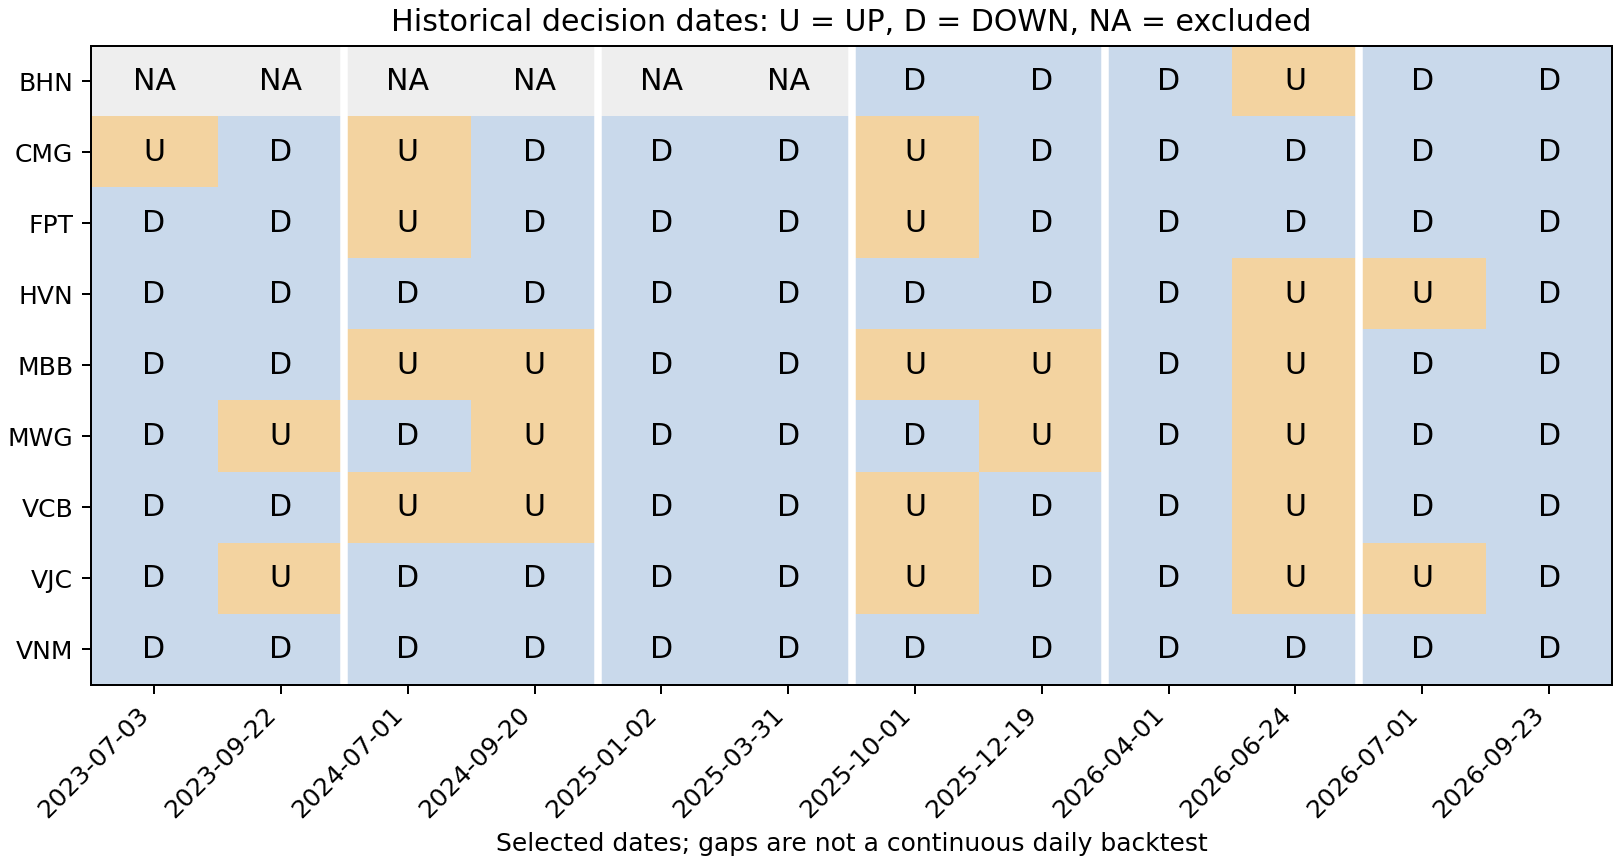
\includegraphics[width=\textwidth]{figs/final_calendar.png}
\caption{Selected historical decision dates and eligibility across nine equities. Missing BHN cells remain excluded rather than being filled with CASH predictions. Labels are shared evaluation truth, not a visualization selected from Full's successful forecasts.}
\label{fig:calendar}
\end{figure}
\begin{table}[p]
\centering\small
\setlength{\tabcolsep}{3pt}
\renewcommand{\arraystretch}{1.15}
\caption{Evaluation scopes and prompt variants in the frozen historical study. Shared main/upstream executions are counted once.}
\label{tab:scope}
\textbf{A. Recorded supports}\par\smallskip
\begin{tabular}{lrrrrrrr}
\hline
Scope & $N$/exec. & Symbols & Dates & Blocks & UP/DOWN & Exec. & Decisions \\
\hline
Main & 102 & 9 & 12 & 6 & 25/77 & 1 & 204 \\
Upstream & 9 & 9 & 3 & 3 & 2/7 & 3 & 54 \\
Factorial & 9 & 8 & 4 & 3 & 2/7 & 3 & 135 \\
\hline
\end{tabular}\par\medskip
\textbf{B. Prompt sections}\par\smallskip
\begin{tabular}{llll}
\hline
Variant & Factors & Sentiment & Representation \\
\hline
B & -- & -- & Shared price reports \\
A & Current & -- & Five-row factorial \\
S & -- & Current & Factorial \\
AS & Current & Current & Compact main / five-row factorial \\
P & Past donor & Current & Five-row factorial \\
\hline
\end{tabular}\par\medskip
\begin{minipage}{\textwidth}\footnotesize Main uses B/AS; upstream uses B/AS; factorial uses B/A/S/AS/P. Class counts are per execution. Upstream includes 18 main r0 calls: 204+54+135-18=375 unique Decisions. P preserves current names/schema/missingness and sentiment, replacing factor values/signals/skill metadata by one past train-only rank-vector donor.\end{minipage}
\end{table}


\begin{figure}[!htbp]
\centering\begin{tikzpicture}[x=1cm,y=1cm,>=Latex,
 box/.style={draw=blue!55!black,fill=blue!4,rounded corners,align=center,text width=4.1cm,minimum height=1.5cm,font=\footnotesize},arr/.style={->,thick}]
\draw[->,thick] (-0.3,0)--(14.5,0);
\node[font=\footnotesize] at (7.1,-0.9) {Observed bar position};
\draw[very thick,blue!60!black] (0,0.2)--(8.4,0.2);
\node[above,align=center,font=\small] at (4.2,0.3) {Chart window $[e-45,e)$\\Only bars through decision $d=e-1$ are visible};
\foreach \x/\lab in {0/{e-45},8.4/{d=e-1},10/{e},13.6/{e+2}}{\draw (\x,-0.12)--(\x,0.12);\node[below,font=\small] at (\x,-0.15) {$\lab$};}
\draw[<->,thick,orange!80!black] (10,1.5)--(13.6,1.5);
\node[above,align=center,font=\small] at (11.8,1.6) {Entry Open to exit Close\\$L=3$ observed bars};
\node[box] (t) at (2,-2.5) {Chronological training\\Labels mature before validation};
\node[box] (v) at (7.1,-2.5) {Validation / purge\\Labels exit before first test decision};
\node[box] (q) at (12.2,-2.5) {Frozen test dates\\Two dates per block; six blocks};
\draw[arr] (t)--(v);\draw[arr] (v)--(q);
\node[align=center,text width=14.0cm,font=\footnotesize] at (7.1,-4.5) {Shared reports $\rightarrow$ variant Decisions $\rightarrow$ immutable truth and separate accounts.\\Twelve dates / 102 eligible units; no synthetic bars and no uniform $S=3$ grid.};
\end{tikzpicture}

\caption{Walk-forward time-index and split contract. The 45-bar chart ends at $d=e-1$, entry is at $e$ and the $L=3$ target is at $e+2$. The final study visits twelve selected dates across six blocks; it does not use a uniform $S=3$, twenty-point grid. Outer cutoff isolation does not certify native row-wise causality.}
\label{fig:walkforward}
\end{figure}

\subsection{Paired Baseline and Disentangled Ablations}
All nine classifiers use the same 102 main units and net target. CASH and always-LONG are constant predictions; always-LONG closes and pays costs every cycle. Train-majority uses purged training labels, choosing CASH on a tie. Momentum predicts LONG for a strictly positive trailing 20-session return. Logistic-price uses numerical price features; logistic-matched adds the recorded factor/sentiment/missingness inputs. Imputation, scaling, regularization and decision threshold selection follow chronological train/validation rules; final logistic refits use matured train plus validation only. We reuse their saved predictions rather than refitting after observing outcomes. The fixed factor-vote comparator uses training-fitted medians/orientation and differs from the native top-five policy and the auxiliary numeric-control study.

Matched numerical inputs do not equal chart images, report wording or pretrained knowledge. Full--Base differences likewise include prompt structure, report length and propensity to choose CASH. The upstream panel has nine units, B/AS and three regenerated upstream realizations with a Decision execution per realization. The factorial panel has nine different-support units, B/A/S/AS/P and three Decision executions with fixed upstream. Both have two UP/seven DOWN per execution, but only the former covers nine symbols. We do not infer main-grid variability or separate upstream/Decision variance components from their SDs.

P retains current factor names, headings, schema/missingness and sentiment, replacing scalar values, signals and skill fields using a predetermined earlier train-only rank-vector donor. Donor label exits precede validation/test. Rank mapping is not name-matched covariance preservation, a placebo distribution or exposure matching. Five explicit rows reach each A/AS/P factorial prompt. Main/upstream compact prompts are a separate representation family. Interaction is defined as $AS-A-S+B$; the observed best-single gap $AS-\max(A,S)$ is a different, post-hoc diagnostic and not an eighth factorial contrast.

\subsection{Account and Statistical Metrics}
BA averages UP and DOWN recall; MCC and both-class precision/recall accompany ordinary accuracy and LONG rate. Pooled metrics retain actual class supports. Symbol macro means are unweighted and report planned/defined denominators. Missing class support or a degenerate MCC denominator yields NA, not zero. Main contrasts use 10,000 paired whole-block resamples, seed 20261102, retaining dates, cross-section, variants and eligibility together. Repeat diagnostics jointly resample recorded blocks and paired execution indices. Intervals condition on finite draws; undefined counts remain visible. Circular block lengths, leave-one-block-out and Bartlett HAC at lags 0/1/2 are sensitivity diagnostics. HAC uses calendar-aligned accuracy differences in fixed-universe panels, with a $t(n_{dates}-1)$ reference; few clusters, irregular gaps and post-inference additions prevent calibrated significance or power claims.

To specify the classification estimand, let TP/FN count UP outcomes and TN/FP count DOWN outcomes. We use
\begin{equation}
 \begin{aligned}
 BA&=\frac12\left(\frac{TP}{TP+FN}+\frac{TN}{TN+FP}\right),\\
 MCC&=\frac{TP\,TN-FP\,FN}{\sqrt{(TP+FP)(TP+FN)(TN+FP)(TN+FN)}}.
 \end{aligned}
 \label{eq:classification_metrics}
\end{equation}
The relevant metric is undefined when a required denominator is zero. Macro means average defined symbol-level values while retaining the planned and defined denominators. A CASH rule can have high ordinary accuracy in a DOWN-heavy sample without discriminating the two classes.

Each of 51 symbol--block accounts starts with VND50 million, without cross-symbol capital competition. LONG follows Eq.~\ref{eq:netlabel}; CASH stays flat. Continuous hold buys once from the first entry through the last scheduled exit, including gaps, and is not a tenth classifier. Wealth includes pending receivables and residual shares at recorded mark-to-market prices. Daily-close drawdown uses an initial-capital anchor. Where supplied in companions, daily Sharpe uses population SD and a 252-session convention with zero risk-free rate; the retained Sortino convention uses SD of negative daily observations, not downside RMS. Annualised cycle ratios are NA for the irregular/gapped main schedules, and are not presented as investment-quality estimates from a handful of trades.

The reference assumes fractional fills at recorded prices and two-leg fees/slippage. Shares are assumed sellable in the afternoon of T+2 conditional on allocation and fill; sale proceeds are pending until the specified settlement phase. This convention follows the archived settlement source \cite{vsd2022settlement}. L=3 is a fixed observed-bar protocol choice, not an optimized horizon. Daily OHLC cannot authenticate opening-auction queues, price-limit fills, partial fills or correct volume units. All twelve sensitivities, including pending cash, advances, cost changes, sell charge, no-fill/delay proxies and lot/capacity assumptions, remain in \ref{app:additional}. Venue/calendar review flags, including ten HVN unit flags, are retained rather than converted to certified fills or synthetic CASH.

\subsection{Implementation and Robustness Design}
Archived SDK aliases are \texttt{openai/gpt-oss-20b} for text and \texttt{qwen/qwen3.8-27b} for vision. Configured temperature zero appears as $10^{-8}$ in observed SDK metadata; no hosted decoding seed is recorded. Text/vision output caps are 2,048/1,024 tokens. Retry/checkpoint records preserve individual attempts and completed outputs. Aliases and 40 response fingerprints do not authenticate an immutable weight revision or historical provider catalogue; 91 original Pattern requests lack epoch/provider-org fields and remain unknown. Offline replay reproduces saved-prediction metrics, not a fresh hosted inference experiment.

The closure contains 649 attempts, 615 successes and 34 errors, including 120 original Pattern calls replayed as shared dependencies. Observed usage totals 1,063,328 prompt and 340,736 completion tokens. Error usage/latency and monetary billing are unknown. Pattern tokens/latency describe original calls, not replay lookup cost; successful callback elapsed times are not wall-clock runtime. Full accounting, pins and hashes are in repository artifacts rather than an implementation appendix.

\section{Backtest Results}
\label{sec:backtestresults}

\subsection{Nine-Symbol Paired Benchmark}

The original 180 net labels contain 56 UP and 124 DOWN outcomes. Full has
confusion counts TP/FN/TN/FP of 16/40/101/23, compared with 15/41/77/47 for
Base reports. Its 65.0\% accuracy is below constant DOWN/CASH at 68.9\%.
Full's balanced accuracy is 55.01\% and MCC is 0.113; the Base reports values
are 44.44\% and $-0.108$. Full issues 39 LONG calls versus 62 for Base reports.
Of 25 additional correct Full decisions, 24 are DOWN and one is UP. This
pattern is consistent with fewer LONG decisions in a predominantly
unprofitable-cycle sample, but does not identify the cause as alpha information.
Tables~\ref{tab:r1_legacy_metrics} and \ref{tab:r1_class_metrics} report the
imbalance-aware audit without suppressing the stronger constant baseline.

\begin{table}[!htb]
\centering
\small
\caption{Legacy class-imbalance audit on the original 180 labels and cycle endpoints.}
\label{tab:r1_legacy_metrics}
\setlength{\tabcolsep}{6pt}
\renewcommand{\arraystretch}{1.12}
\setbox0=\hbox{%
\begin{tabular}{lrrrrrrr}
\hline
Variant & $N$ & Acc. (\%) & BA (\%) & MCC & Macro-F1 (\%) & LONG (\%) & Mean return (\%) \\
\hline
Full (legacy) & 180 & 65.00 & 55.01 & 0.113 & 54.96 & 21.67 & -1.68 \\
Base reports (legacy) & 180 & 51.11 & 44.44 & -0.108 & 44.53 & 34.44 & -8.43 \\
Constant DOWN / CASH & 180 & 68.89 & 50.00 & NA & 40.79 & 0.00 & 0.00 \\
Always-LONG cycles & 180 & 31.11 & 50.00 & NA & 23.73 & 100.00 & -17.69 \\
\hline
\end{tabular}}
\ifdim\wd0>0.98\textwidth\resizebox{0.98\textwidth}{!}{\copy0}\else\copy0\fi
\par\smallskip
\begin{minipage}{0.98\textwidth}\footnotesize Predictive metrics are pooled; return is the mean of nine independent accounts, not a pooled portfolio. UP/DOWN support is 56/124. Undefined values are NA. Always-LONG closes and reopens each cycle; it is not buy-and-hold.\end{minipage}
\end{table}

\begin{table}[!htb]
\centering
\small
\caption{Per-class legacy precision, recall and F1, in percent.}
\label{tab:r1_class_metrics}
\setlength{\tabcolsep}{6pt}
\renewcommand{\arraystretch}{1.12}
\setbox0=\hbox{%
\begin{tabular}{llrrrr}
\hline
Variant & Class & Support & Precision & Recall & F1 \\
\hline
Full (legacy) & UP & 56 & 41.03 & 28.57 & 33.68 \\
Full (legacy) & DOWN & 124 & 71.63 & 81.45 & 76.23 \\
Base reports (legacy) & UP & 56 & 24.19 & 26.79 & 25.42 \\
Base reports (legacy) & DOWN & 124 & 65.25 & 62.10 & 63.64 \\
Constant DOWN / CASH & UP & 56 & NA & 0.00 & 0.00 \\
Constant DOWN / CASH & DOWN & 124 & 68.89 & 100.00 & 81.58 \\
Always-LONG cycles & UP & 56 & 31.11 & 100.00 & 47.46 \\
Always-LONG cycles & DOWN & 124 & NA & 0.00 & 0.00 \\
\hline
\end{tabular}}
\ifdim\wd0>0.98\textwidth\resizebox{0.98\textwidth}{!}{\copy0}\else\copy0\fi
\par\smallskip
\begin{minipage}{0.98\textwidth}\footnotesize A class with support but no predicted positives has undefined precision and zero recall/F1. All symbol-level confusion matrices and class metrics are retained in the reanalysis CSV/JSON.\end{minipage}
\end{table}


Table~\ref{tab:overall_results} retains the historical paired summaries for
traceability. Its Full--Base gap is a bundle comparison. Stored cross-symbol
Wilcoxon and small-sample intervals are descriptive legacy diagnostics, not
evidence of a general significant alpha or forecasting improvement.

\begin{table}[!htb]
\centering
\caption{Paired benchmark over nine equities ($N=20$ per symbol, $W=45$, $S=3$, $L=3$). Panel A reports directional inference; Panel B reports compounded long-only account outcomes.}
\label{tab:overall_results}
\renewcommand{\arraystretch}{1.12}
\setlength{\tabcolsep}{3.2pt}
\footnotesize

\textit{Panel A: Directional accuracy and paired inference}

\resizebox{0.95\columnwidth}{!}{%
\begin{tabular}{lrrrrrr}
\hline
\textbf{Symbol} & \textbf{Full (\%)} & \textbf{No-$\alpha$ (\%)} & \textbf{Lift (pp)} & \textbf{95\% CI (pp)} & \textbf{McNemar $p$} & \textbf{$N$} \\
\hline
BHN & 55.0 & 45.0 & +10.0 & $[+0.0,+15.0]$ & 0.6875 & 20 \\
CMG & 75.0 & 70.0 & +5.0 & $[+0.0,+5.0]$ & 1.0000 & 20 \\
FPT & 65.0 & 45.0 & +20.0 & $[-5.0,+35.0]$ & 0.2188 & 20 \\
HVN & 70.0 & 50.0 & +20.0 & $[+0.0,+35.0]$ & 0.2188 & 20 \\
MBB & 70.0 & 45.0 & +25.0 & $[+0.0,+55.0]$ & 0.1250 & 20 \\
MWG & 70.0 & 50.0 & +20.0 & $[+0.0,+40.0]$ & 0.1250 & 20 \\
VCB & 65.0 & 50.0 & +15.0 & $[+5.0,+35.0]$ & 0.2500 & 20 \\
VJC & 60.0 & 60.0 & +0.0 & $[-10.0,+10.0]$ & 1.0000 & 20 \\
VNM & 55.0 & 45.0 & +10.0 & $[-15.0,+45.0]$ & 0.6250 & 20 \\
\hline
\textbf{Mean / total N} & \textbf{65.0} & \textbf{51.1} & \textbf{+13.9} & -- & -- & \textbf{180} \\
\hline
\end{tabular}}

\vspace{0.7em}
\textit{Panel B: Compounded account metrics}
\footnotesize

\resizebox{0.95\columnwidth}{!}{%
\begin{tabular}{lrrrrrr}
\hline
\textbf{Symbol} & \textbf{Return F (\%)} & \textbf{Return N (\%)} & \textbf{Sharpe F} & \textbf{Sharpe N} & \textbf{MDD F (\%)} & \textbf{MDD N (\%)} \\
\hline
BHN & -4.20 & -5.76 & -3.63 & -2.64 & 4.80 & 8.31 \\
CMG & -2.66 & -5.60 & -3.64 & -5.28 & 2.66 & 5.60 \\
FPT & -1.56 & -10.37 & -0.86 & -6.41 & 6.30 & 10.37 \\
HVN & +2.89 & -15.64 & +1.19 & -4.27 & 5.27 & 20.06 \\
MBB & +5.21 & -7.78 & +2.36 & -4.22 & 3.50 & 9.89 \\
MWG & +0.39 & -6.42 & +0.41 & -3.93 & 1.92 & 8.17 \\
VCB & -8.34 & -10.49 & -5.98 & -7.78 & 8.92 & 10.49 \\
VJC & -6.05 & -6.26 & -5.22 & -5.38 & 6.05 & 6.26 \\
VNM & -0.85 & -7.51 & -0.41 & -4.91 & 3.40 & 7.51 \\
\hline
\textbf{Mean} & \textbf{-1.69} & \textbf{-8.43} & \textbf{-1.75} & \textbf{-4.98} & \textbf{4.76} & \textbf{9.63} \\
\hline
\end{tabular}}

\vspace{0.4em}
\begin{flushleft}\footnotesize
F and N denote Full and No-Alpha. The 95\% intervals use a moving-block bootstrap (block length 5; 1,000 replications). The two-sided cross-symbol Wilcoxon result is $p=0.0078125$ (nine symbol-level lifts; median lift $=15.0$ pp). Returns are compounded from VND~50,000,000 independent accounts under Eq.~\eqref{eq:account_return}; SHORT forecasts remain in cash.
\end{flushleft}
\end{table}

Full's recomputed mean account return is $-1.6833\%$; averaging the already
rounded legacy percentages instead gives $-1.6856\%$, explaining the historical
$-1.69\%$ display. Both are below CASH at zero. These are means of nine
independent accounts, not a joint portfolio. Correct SHORT predictions earn no
return under the long-only map. Neither the Full--Base accuracy gap nor
relative loss reduction establishes isolated alpha value or profitability.

\subsection{Numerical Reconstruction and Daily Ledgers}

Tables~\ref{tab:r1_numeric_metrics} and \ref{tab:r1_comparability} report the
additional numerical study under Section~\ref{sec:r1_numeric_protocol}.
These results belong to the new snapshot and are not ranked against Full's
legacy outcomes. The price-only and factor-augmented logistic models answer
different information-set questions; neither has verified identical archived
Full reports. The continuous-hold account buys once and sells once, unlike
always-LONG cycles. Daily-close drawdown, turnover, fees and exposure are
retained per symbol in the reanalysis ledgers; no daily Full ledger is inferred
from mismatched reconstructed prices. The train-rate random control is not
represented as matching Full's exposure. Accordingly, the newly implemented
baselines do not by themselves close the common-snapshot and same-information
requirements of a confirmatory baseline comparison.

\begin{table}[!htb]
\centering
\small
\caption{Exploratory numerical baselines on the newly retrieved snapshot: not a head-to-head comparison with legacy Full.}
\label{tab:r1_numeric_metrics}
\setlength{\tabcolsep}{6pt}
\renewcommand{\arraystretch}{1.12}
\setbox0=\hbox{%
\begin{tabular}{lrrrrrr}
\hline
Variant & Acc. (\%) & BA (\%) & MCC & Mean return (\%) & Mean daily MDD (\%) & Held sessions (\%) \\
\hline
Constant DOWN / CASH & 68.89 & 50.00 & NA & 0.00 & 0.00 & 0.00 \\
Always-LONG cycles & 31.11 & 50.00 & NA & -17.33 & 21.13 & 99.15 \\
Continuous hold (price only) & NA & NA & NA & -5.53 & 14.74 & 100.00 \\
Factor-only vote & 61.67 & 62.38 & 0.230 & -5.07 & 11.93 & 46.75 \\
Logistic: price & 66.11 & 52.88 & 0.077 & -1.15 & 4.22 & 13.80 \\
Logistic: price + factors + S/M & 61.67 & 51.12 & 0.025 & -2.83 & 7.38 & 21.62 \\
Momentum (20) & 50.00 & 46.08 & -0.074 & -8.55 & 10.50 & 40.60 \\
Train majority & 68.89 & 50.00 & NA & 0.00 & 0.00 & 0.00 \\
Train-rate random control & 50.56 & 47.47 & -0.047 & -10.03 & 12.06 & 42.44 \\
\hline
\end{tabular}}
\ifdim\wd0>0.98\textwidth\resizebox{0.98\textwidth}{!}{\copy0}\else\copy0\fi
\par\smallskip
\begin{minipage}{0.98\textwidth}\footnotesize All cycle classifiers use the same 180 new-snapshot cutoffs and net targets. Predictive metrics are pooled; economic columns average independent symbol accounts. S/M denotes verified sentiment and missingness; historical scorer provenance is unavailable, so sentiment scores are missing. The train-rate control uses training momentum exposure, not Full exposure. Continuous hold has one buy and one sell per symbol; price adjustments and dividends are not independently certified. No Full row is included because 74 cycles differ at entry and/or exit from legacy, including two changed labels.\end{minipage}
\end{table}

\begin{table}[!htb]
\centering
\small
\caption{Training support and snapshot comparability audit.}
\label{tab:r1_comparability}
\setlength{\tabcolsep}{6pt}
\renewcommand{\arraystretch}{1.12}
\setbox0=\hbox{%
\begin{tabular}{lrrrrr}
\hline
Symbol & Train & Validation & Test & Different endpoints & Label changes \\
\hline
BHN & 175 & 34 & 20 & 20 & 2 \\
CMG & 399 & 36 & 20 & 1 & 0 \\
FPT & 399 & 36 & 20 & 20 & 0 \\
HVN & 399 & 36 & 20 & 1 & 0 \\
MBB & 399 & 36 & 20 & 1 & 0 \\
MWG & 399 & 36 & 20 & 20 & 0 \\
VCB & 399 & 36 & 20 & 9 & 0 \\
VJC & 399 & 36 & 20 & 0 & 0 \\
VNM & 399 & 36 & 20 & 2 & 0 \\
\hline
\end{tabular}}
\ifdim\wd0>0.98\textwidth\resizebox{0.98\textwidth}{!}{\copy0}\else\copy0\fi
\par\smallskip
\begin{minipage}{0.98\textwidth}\footnotesize Each label exit precedes the next split's first decision. BHN uses a valid suffix beginning 14 September 2022 after an unverified OHLC contradiction; raw data are preserved. All 20 test dates are retained for every symbol. Matching aggregate class counts does not establish matching labels or snapshots.\end{minipage}
\end{table}


\subsection{Robustness and Sensitivity}

Table~\ref{tab:robustness_results} reports all six completed sweeps. Each row contains 20 paired test points. Panel A changes the input window for both variants and therefore changes the No-Alpha information set. In Panels B and C, which intervene only on Alpha processing, the No-Alpha accuracy is exactly invariant within each symbol and panel: 45.0\% for both normalisation sweeps, 50.0\% for the FPT weight sweep, and 45.0\% for the VNM weight sweep.

\begin{table}[!htb]
\centering
\caption{Robustness sweep on FPT and VNM ($N=20$ per row). Returns are compounded account returns.}
\label{tab:robustness_results}
\renewcommand{\arraystretch}{1.08}
\setlength{\tabcolsep}{2.8pt}
\resizebox{\columnwidth}{!}{%
\begin{tabular}{lllrrrrr}
\hline
\textbf{Symbol} & \textbf{Panel} & \textbf{Scenario} & \textbf{Full (\%)} & \textbf{No-$\alpha$ (\%)} & \textbf{Lift (pp)} & \textbf{Return F (\%)} & \textbf{Return N (\%)} \\
\hline
FPT & Window & $W=30$ & 55.0 & 40.0 & +15.0 & -2.63 & -10.27 \\
FPT & Window & $W=45$ & 65.0 & 50.0 & +15.0 & -2.21 & -6.86 \\
FPT & Window & $W=60$ & 40.0 & 45.0 & -5.0 & -8.04 & -4.38 \\
VNM & Window & $W=30$ & 40.0 & 40.0 & +0.0 & -7.81 & -7.51 \\
VNM & Window & $W=45$ & 55.0 & 40.0 & +15.0 & -3.59 & -7.06 \\
VNM & Window & $W=60$ & 65.0 & 55.0 & +10.0 & +5.20 & -0.84 \\
\hline
FPT & Normalisation & \texttt{zscore\_tanh} & 50.0 & 45.0 & +5.0 & -4.72 & -7.38 \\
FPT & Normalisation & \texttt{minmax} & 55.0 & 45.0 & +10.0 & -5.63 & -7.38 \\
FPT & Normalisation & \texttt{rank} & 60.0 & 45.0 & +15.0 & -4.36 & -7.38 \\
VNM & Normalisation & \texttt{zscore\_tanh} & 60.0 & 45.0 & +15.0 & +2.70 & -2.22 \\
VNM & Normalisation & \texttt{minmax} & 65.0 & 45.0 & +20.0 & +3.89 & -2.22 \\
VNM & Normalisation & \texttt{rank} & 55.0 & 45.0 & +10.0 & -2.01 & -2.22 \\
\hline
FPT & Weighting & \texttt{default} & 60.0 & 50.0 & +10.0 & -1.99 & -7.85 \\
FPT & Weighting & \texttt{equal\_weight} & 60.0 & 50.0 & +10.0 & -0.36 & -7.85 \\
FPT & Weighting & \texttt{ic\_heavy} & 65.0 & 50.0 & +15.0 & -2.21 & -7.85 \\
VNM & Weighting & \texttt{default} & 65.0 & 45.0 & +20.0 & +6.17 & -5.19 \\
VNM & Weighting & \texttt{equal\_weight} & 50.0 & 45.0 & +5.0 & -4.57 & -5.19 \\
VNM & Weighting & \texttt{ic\_heavy} & 60.0 & 45.0 & +15.0 & +2.70 & -5.19 \\
\hline
\end{tabular}}
\end{table}

The stored alpha-enabled branch varies with configuration. These sweeps do not validate historical branch provenance or establish alpha information value: snapshot dates differ between experiments, repeats are absent, and the control may be weak. Their arithmetic is retained for traceability, while substantive robustness conclusions await a verified common-snapshot study.

\subsection{Disentangled Alpha--Sentiment Ablation}

Table~\ref{tab:disentangled_ablation} retains the legacy four-way summaries for traceability only. Identical prediction sequences across differently labelled FPT branches and missing request archives leave provenance unresolved. The numerical gaps in this table therefore cannot be called independent alpha or sentiment contributions. Its final column is the stored improvement over the best single component, not the factorial interaction.

\begin{table}[!htb]
\centering
\caption{Unverified legacy four-way summaries ($N=20$ per variant and symbol); not confirmatory attribution evidence.}
\label{tab:disentangled_ablation}
\renewcommand{\arraystretch}{1.1}
\setlength{\tabcolsep}{3pt}

\textit{Panel A: Directional decomposition}

\resizebox{\columnwidth}{!}{%
\begin{tabular}{lrrrrrrr}
\hline
\textbf{Symbol} & \textbf{Full} & \textbf{Alpha-only} & \textbf{Sent.-only} & \textbf{Baseline} & \textbf{$\Delta\alpha$} & \textbf{$\Delta$Sent.} & \textbf{Synergy} \\
\hline
FPT & 55.0\% & 50.0\% & 45.0\% & 45.0\% & +5.0 pp & +0.0 pp & +5.0 pp \\
VNM & 60.0\% & 50.0\% & 50.0\% & 45.0\% & +5.0 pp & +5.0 pp & +10.0 pp \\
VCB & 45.0\% & 55.0\% & 40.0\% & 40.0\% & +15.0 pp & +0.0 pp & -10.0 pp \\
\hline
\textbf{Mean} & \textbf{53.33\%} & \textbf{51.67\%} & \textbf{45.00\%} & \textbf{43.33\%} & \textbf{+8.33 pp} & \textbf{+1.67 pp} & \textbf{+1.67 pp} \\
\hline
\end{tabular}}

\vspace{0.7em}
\textit{Panel B: Compounded account return}

\begin{tabular}{lrrrr}
\hline
\textbf{Symbol} & \textbf{Full} & \textbf{Alpha-only} & \textbf{Sentiment-only} & \textbf{Baseline} \\
\hline
FPT & -4.61\% & -7.85\% & -7.38\% & -6.09\% \\
VNM & -4.03\% & +2.26\% & -5.86\% & -3.96\% \\
VCB & -7.93\% & -2.75\% & -9.23\% & -11.34\% \\
\hline
\end{tabular}
\end{table}

No component-information conclusion is drawn from these unverified summaries. Their presence preserves the audit trail; replacing them as confirmatory evidence requires verified factorial/placebo branches on common data and repeated runs, rather than interpreting arithmetic differences as information value.

\section{Discussion and limitations}
\label{sec:limitations}

\paragraph{What the comparisons establish}
The archived implementation yields identifiable forecasts and replayable metrics, but its Full--Base contrast changes a bundle of inputs and prompt structure. Main/upstream compact reports differ from explicit factorial values. Matching report parents or numerical inputs does not match text/image representations, pretrained knowledge, exposure or semantic use. The rank-vector placebo tests one predetermined past replacement, not a distribution of independent placebo treatments. Consequently, these results describe recorded behaviour and do not isolate causal alpha, sentiment or selector value. Byte-level duplication in legacy artifacts is audited rather than treated as proof that historical branch labels were correct; those legacy ablations no longer support component attribution.

\paragraph{Causal construction and domain validity}
The native row-wise causal failure in Section~\ref{sec:formulation} remains unresolved in the frozen study. Its in-sample ranking/orientation and heuristic expression translations limit any factor-discovery interpretation. The numerical controls use a separate causal path, so their passing probes cannot certify the earlier native inputs. Similarly, saved scorer probabilities, a pinned local checkpoint and strict date rules cannot authenticate the original news content or publication availability. No independent financial-domain labels, agreement/adjudication or domain test performance are available. Missing sentiment is not evidence that sentiment was neutral, and rescoring is not validation. Repairing these defects for a new experiment would require versioned inputs and a new protocol, not rewriting old predictions.

\paragraph{Sampling, dependence and hosted variability}
The universe is purposive and potentially survivor-biased; point-in-time listing/delisting/suspension membership is unverified. All outcome dates precede the November 2026 freeze, so model training contamination remains possible even if a named model was publicly released before some test dates. Twelve dates and six blocks, plus three executions on each small panel, do not establish generalization, effective sample size or calibrated uncertainty. Repeats, correlated symbols, overlapping cohorts and repeated bootstrap draws are not extra independent markets. Order deviations, epoch/routing changes and unknown immutable served weights further confound distributional comparisons. The historical scope amendment makes this an exploratory study rather than an untouched confirmatory evaluation.

\paragraph{Economic and visual scope}
Negative account means do not demonstrate a deployable strategy. Reference fills, fee/slippage, settlement phases, lot/capacity limits and volume units are assumptions or proxies, while corporate-action adjustments, price-limit queues, actual spread/depth and partial fills are unauthenticated. Separate account averaging omits portfolio capital competition. L=3 is not optimized. Visual byte/pixel/legend integrity and deterministic consistency flags do not show that the VLM read the claimed candle or trendline; matched counterfactual charts and local-evidence annotation would be needed to test that stronger claim. Prompt precedence is not a learned or guaranteed conflict-resolution mechanism.

\paragraph{Next evidence and responsible interpretation}
A prospective versioned study should repair native row causality, repeat selection/preprocessing inside chronological training, and preserve a later untouched evaluation interval. Candidate search can be assessed with procedures such as White's Reality Check or a Deflated Sharpe analysis \cite{white2000reality,bailey2014deflated}; neither is claimed as completed here. Independent financial-news labels and human visual-evidence annotations are needed before domain/semantic reliability claims. More calendar coverage and controlled repeated hosted calls would be required for stable model/component conclusions; executable portfolio validation needs separately authenticated market and settlement information. Public release is also conditional on rights and a real archive identifier. These are outstanding requirements, not benefits inferred from the current experiment. The implementation is research decision support and should not be represented as profitable trading advice.

\section{Conclusion}
\label{sec:conclusion}

This reanalysis documents the evidence limits of a five-agent decision-support implementation for Vietnamese equities. The legacy Full branch achieves 65.0\% raw accuracy, below the 68.9\% constant DOWN/CASH benchmark, and has a negative mean account return. Balanced accuracy of 55.0\% and MCC of 0.113 describe modest class-balanced discrimination in this single archived run, without establishing superiority or a reliable alpha effect. The weaker Base reports control also removes sentiment, so its comparison with Full cannot identify alpha information value.

The numerical reconstruction adds train-fitted majority, momentum, two logistic feature sets and factor-only baselines, with explicit preprocessing and daily ledgers. However, 74 of the 180 cycles differ from legacy and two individual labels change. These results therefore remain a separate exploratory analysis. Archived Full training predictions and complete report/feature inputs are still unavailable for a genuine Full-exposure-matched and identical-information comparison. Predictive superiority, isolated alpha/sentiment value and profitability are not established. Recovering the authenticated historical inputs or performing a newly frozen common-snapshot evaluation is required before those claims can be reconsidered; software checks and revised presentation alone do not complete that evidentiary requirement.


%% CRediT authorship contribution statement
%% (elsarticle.cls has no \credit/\printcredits macros; the CRediT
%% roles from the original cas-sc source are preserved here verbatim
%% as a standard Elsevier "CRediT authorship contribution statement"
%% section instead.)
\section*{CRediT authorship contribution statement}

\textbf{Van-Tang Nguyen:} Conceptualization (C); Software (So); Validation (Va); Investigation (I); Original draft preparation (O); Project administration (P); Funding acquisition (Fu).

\textbf{Hoang-Dung Phan:} Methodology (M); Software (So); Formal analysis (Fo); Investigation (I); Resources (R); Data curation (D); Original draft preparation (O); Writing-review and editing (E); Visualization (Vi); Supervision (Su).

\textbf{Thanh-Tam Do Thi:} Methodology (M); Investigation (I); Data curation (D); Original draft preparation (O); Writing-review and editing (E); Supervision (Su).

\textbf{Phuong-Thai Nguyen:} Methodology (M); Investigation (I); Data curation (D); Original draft preparation (O); Visualization (Vi); Supervision (Su).

\textbf{Hong-Viet Tran:} Conceptualization (C); Methodology (M); Software (So); Validation (Va); Formal analysis (Fo); Data curation (D); Original draft preparation (O); Writing-review and editing (E); Project administration (P).

\section*{CONFLICT OF INTEREST STATEMENT (mandatory)}
Authors state no conflict of interest.

% \section*{INFORMED CONSENT (if applicable)}
% The protection of privacy is a legal right that must not be breached without individual informed consent. In cases where the identification of personal information is necessary for scientific reasons, authors should obtain full documentation of informed consent, including written permission from the patient prior to inclusion in the study. Incorporate the following (or a similar) statement: We have obtained informed consent from all individuals included in this study.

% \section*{ETHICAL APPROVAL (if applicable)}
% When papers talk about using people or animals, authors should make it clear that the research followed all national rules and institutional policies, and it was approved by the authors' institutional review board or a similar committee. The Helsinki Declaration's tenets must guide all investigations involving human subjects. Authors must also identify the committee or review board approving the experiments and provide a statement indicating approval of the research. Incorporate the following (or a similar) statement: The research related to human use has been complied with all the relevant national regulations and institutional policies in accordance with the tenets of the Helsinki Declaration and has been approved by the authors' institutional review board or equivalent committee; or: The research related to animal use has been complied with all the relevant national regulations and institutional policies for the care and use of animals.


\section*{CODE AVAILABILITY}
The source code and demonstration implementation of the proposed framework are available in the \href{https://github.com/DungPhanHoangg05/A-Multi-Agent-Large-Language-Model-Approach-to-Price-Driven-Stock-Trading-in-the-Vietnamese-Stock-Ma.git}{project repository}.

\section*{Acknowledgments}
This research is funded by Foreign Trade University under research program number FTURP02-2026-08


%% ── APPENDIX ──────────────────────────────────────────────────────────────────


\FloatBarrier
\appendix
\setcounter{table}{0}
\section{Signal definitions and implementation distinctions}
\label{app:signals}
The tables retain scientific definitions needed to interpret the implemented reports. Full Python, operator windows/guards, expression registry and complete prompts remain in the companion repository/package. Declared state slots do not imply their numerical arrays reached Decision; the actual Indicator path delivers report text and messages.
\begin{table}[!htbp]
\centering\small
\setlength{\tabcolsep}{3pt}
\renewcommand{\arraystretch}{1.15}
\caption{Indicator signal rules and missing-data conventions.}
\label{tab:indicator_rules}
\textbf{Five deterministic votes}\par\smallskip
\begin{tabular}{lp{7.1cm}p{5.2cm}}
\hline
Signal & Priority and boundaries & Qualification \\
\hline
MACD & Previous strict/current inclusive crossing first; otherwise histogram sign and change. & 12/26/9; no Stochastic histogram. \\
RSI & $\ge70$: bear; $\le30$: bull; $55\le x<70$: bull; $30<x\le45$: bear. & 45--55 uses change against the third retained sample. \\
Stochastic & Crossing precedes $\ge80$ bear / $\le20$ bull; interior fallback retained. & Legacy equality/zero-D truthiness is disclosed. \\
Williams \%R & $\ge-20$: bear; $\le-80$: bull; otherwise retained-sample direction. & Not a volatility vote. \\
ROC & $>+0.5\%$: bull; $<-0.5\%$: bear; equality neutral. & Thresholds follow four-decimal rounding. \\
\hline
\end{tabular}\par\medskip
\begin{minipage}{\textwidth}\footnotesize None/nonfinite values are removed, zero retained; rounding is to four decimals before classification. Retained samples need not be consecutive if missing. Missing/error gives a neutral vote within denominator five. Directional plurality, ties MIXED, and confidence are heuristics, not calibrated probabilities.\end{minipage}
\end{table}

\begin{table}[!htbp]
\centering\small
\setlength{\tabcolsep}{3pt}
\renewcommand{\arraystretch}{1.15}
\caption{Custom native factor definitions and implementation distinctions.}
\label{tab:custom_definitions}
\textbf{Before global normalization and IC orientation}\par\smallskip
\begin{tabular}{lp{8.0cm}p{5.0cm}}
\hline
ID & Native handler expression & Distinction \\
\hline
FDM & $\tanh(0.5\,a_t V_t/ADV_{20,t})$ & Native uses adjusted one-bar return, not the MACD display template. \\
SFA & $\tanh(1.5\tanh(H_t/(0.005C_t+\epsilon))+0.5a_t)$ & Native uses MACD histogram and return, not sentiment; prototype has a distinct sentiment branch. \\
LVR & $\tanh(-0.8\,z_{20}((C_t-SMA_{5,t})/C_t))$ & Rolling mean/SD conventions and partial windows are implementation-specific. \\
BFE & $\tanh(1.5(\%B_t-0.5)\,VolZ_{5,t})$ & Negative VolZ reverses the sign; zero cancels. No squeeze or volume-expansion gate. \\
OFE & $\tanh(3a_t\,CP_t)$ & OHLCV proxy, not measured signed order flow. \\
\hline
\end{tabular}\par\medskip
\begin{minipage}{\textwidth}\footnotesize $a_t$ is one-bar pct-change divided by rolling 20-bar sample SD (minimum five); $H_t$ is MACD(12,26,9) histogram; $CP_t$ is close location relative to the bar midpoint/range; ADV is mean Volume, not dollar volume. Guarded denominators and fills follow the registry. BFE registry sample-SD preprocessing differs from the rounded/population-SD prototype. Six selected metadata slots differ from their handler description, without the literal wrong formula in the affected prompts. A display rank of four does not identify BFE. Full expressions, guards and counterexamples are in the companion registry.\end{minipage}
\end{table}


\FloatBarrier
\setcounter{table}{0}
\section{Additional account and symbol results}
\label{app:additional}
These tables use the same final supports and unchanged predictions as the main results. Supplement S1 gives every baseline by symbol and both classes; S2 contains all execution rows/contrasts; S3 the complete numeric/random family; S4 all temporal/regime/HAC diagnostics. They are scientific companion tables, distinct from raw execution logs and implementation files. No additional market observation is created by these alternative tabulations.
\begin{table}[p]
\centering\small
\setlength{\tabcolsep}{3pt}
\renewcommand{\arraystretch}{1.15}
\caption{Full and Base symbol-level results on their common historical support.}
\label{tab:symbol_results}
\textbf{Percent except MCC}\par\smallskip
\begin{tabular}{lrrrrrr}
\hline
Symbol/variant & UP/DOWN & Acc. & BA & MCC & $R_U$ & $R_D$ \\
\hline
BHN/Full & 1/5 & 100.00 & 100.00 & 1.000 & 100.00 & 100.00 \\
BHN/Base & 1/5 & 66.67 & 80.00 & 0.447 & 100.00 & 60.00 \\
CMG/Full & 3/9 & 66.67 & 44.44 & -0.174 & 0.00 & 88.89 \\
CMG/Base & 3/9 & 75.00 & 61.11 & 0.258 & 33.33 & 88.89 \\
FPT/Full & 2/10 & 66.67 & 40.00 & -0.200 & 0.00 & 80.00 \\
FPT/Base & 2/10 & 50.00 & 30.00 & -0.316 & 0.00 & 60.00 \\
HVN/Full & 2/10 & 66.67 & 60.00 & 0.158 & 50.00 & 70.00 \\
HVN/Base & 2/10 & 66.67 & 60.00 & 0.158 & 50.00 & 70.00 \\
MBB/Full & 5/7 & 50.00 & 48.57 & -0.029 & 40.00 & 57.14 \\
MBB/Base & 5/7 & 58.33 & 55.71 & 0.120 & 40.00 & 71.43 \\
MWG/Full & 4/8 & 58.33 & 56.25 & 0.120 & 50.00 & 62.50 \\
MWG/Base & 4/8 & 50.00 & 50.00 & 0.000 & 50.00 & 50.00 \\
VCB/Full & 4/8 & 58.33 & 50.00 & 0.000 & 25.00 & 75.00 \\
VCB/Base & 4/8 & 50.00 & 37.50 & -0.316 & 0.00 & 75.00 \\
VJC/Full & 4/8 & 58.33 & 43.75 & -0.213 & 0.00 & 87.50 \\
VJC/Base & 4/8 & 50.00 & 37.50 & -0.316 & 0.00 & 75.00 \\
VNM/Full & 0/12 & 83.33 & NA & NA & NA & 83.33 \\
VNM/Base & 0/12 & 83.33 & NA & NA & NA & 83.33 \\
\hline
\end{tabular}\par\medskip
\begin{minipage}{\textwidth}\footnotesize BHN contributes six eligible units, other symbols twelve; NA retains missing-class denominators. S1 additionally contains all nine classifiers for every symbol and both-class precision/recall/F1, with pooled and macro summaries.\end{minipage}
\end{table}

\begin{table}[!htbp]
\centering\small
\setlength{\tabcolsep}{3pt}
\renewcommand{\arraystretch}{1.15}
\caption{All twelve account-execution sensitivities on unchanged predictions.}
\label{tab:execution}
\textbf{Means over 51 accounts per variant}\par\smallskip
\begin{tabular}{lrrrrr}
\hline
Scenario & Base (\%) & Full (\%) & $\Delta$Full (pp) & Stock & Pending \\
\hline
reference & -0.750 & -0.797 & 0.000 & 0 & 0 \\
pending\_t2 & -0.750 & -0.797 & 0.000 & 0 & 0 \\
advance\_on\_demand & -0.750 & -0.797 & 0.000 & 0 & 0 \\
advance\_auto & -0.803 & -0.840 & -0.043 & 0 & 0 \\
lower\_cost & -0.526 & -0.612 & 0.185 & 0 & 0 \\
higher\_cost & -1.249 & -1.211 & -0.414 & 0 & 0 \\
sell\_charge\_10bp & -0.805 & -0.843 & -0.046 & 0 & 0 \\
no\_fill\_proxy & -0.659 & -0.803 & -0.006 & 0 & 0 \\
delayed\_proxy & -0.621 & -0.766 & 0.030 & 0 & 0 \\
lot100\_cap1pct & -0.602 & -0.745 & 0.052 & 0 & 0 \\
combined & -1.074 & -1.166 & -0.369 & 0 & 0 \\
all\_entries\_missed & 0.000 & 0.000 & 0.797 & 0 & 0 \\
\hline
\end{tabular}\par\medskip
\begin{minipage}{\textwidth}\footnotesize Stock/Pending count Full accounts with residual shares/receivables; zero Full residuals do not imply none for other strategies. All 6,120 account executions are in the companion results. Fee/slippage, advance fees, sell charge, lots and capacity are assumptions. No-fill/delay proxies do not measure queue fills; all entries missed is not a mathematical worst bound.\end{minipage}
\end{table}

\FloatBarrier


%% Loading bibliography style file
\bibliographystyle{elsarticle-num}

%% Loading bibliography database
\bibliography{references}

\clearpage

\end{document}
